%# -*- coding: utf-8-unix -*-
%%==================================================
%% thesis.tex
%%==================================================

% 双面打印
\documentclass[master, fontset=adobe, openright, twoside, zihao=-4, review]{sjtuthesis}
% \documentclass[bachelor, fontset=adobe, openany, oneside, submit]{sjtuthesis}
% \documentclass[master, fontset=adobe, review]{sjtuthesis}
% \documentclass[%
%   bachelor|master|doctor,	% 必选项
%   fontset=adobe|windows,  	% 只测试了adobe
%   oneside|twoside,		% 单面打印,双面打印(奇偶页交换页边距,默认)
%   openany|openright, 		% 可以在奇数或者偶数页开新章|只在奇数页开新章(默认)
%   zihao=-4|5,, 		% 正文字号:小四、五号(默认)
%   review,	 		% 盲审论文,隐去作者姓名、学号、导师姓名、致谢、发表论文和参与的项目
%   submit			% 定稿提交的论文,插入签名扫描版的原创性声明、授权声明 
% ]

% 逐个导入参考文献数据库
\addbibresource{bib/thesis.bib}
% \addbibresource{bib/chap2.bib}

\begin{document}

%% 无编号内容:中英文论文封面、授权页
%# -*- coding: utf-8-unix -*-
\title{面向软件定义存储的云混合存储技术研究}
\author{李然}
\advisor{陈昊鹏副教授}
% \coadvisor{某某教授}
\defenddate{2018年1月5日}
\school{上海交通大学}
\institute{电子信息与电气工程学院}
\studentnumber{115037910067}
\major{软件工程}

\englishtitle{Research on Software Defined Storage on Cloud Hybrid Storage Technique}
\englishauthor{\textsc{Ran Li}}
\englishadvisor{Prof. \textsc{Haopeng Chen}}
% \englishcoadvisor{Prof. \textsc{Uom Uom}}
\englishschool{Shanghai Jiao Tong University}
\englishinstitute{\textsc{School of Software Engineering} \\
  \textsc{Shanghai Jiao Tong University} \\
  \textsc{Shanghai, P.R.China}}
\englishmajor{Software Engineering}
\englishdate{Jan. 5th, 2018}


\maketitle

\makeenglishtitle

\makeatletter
\ifsjtu@submit\relax
	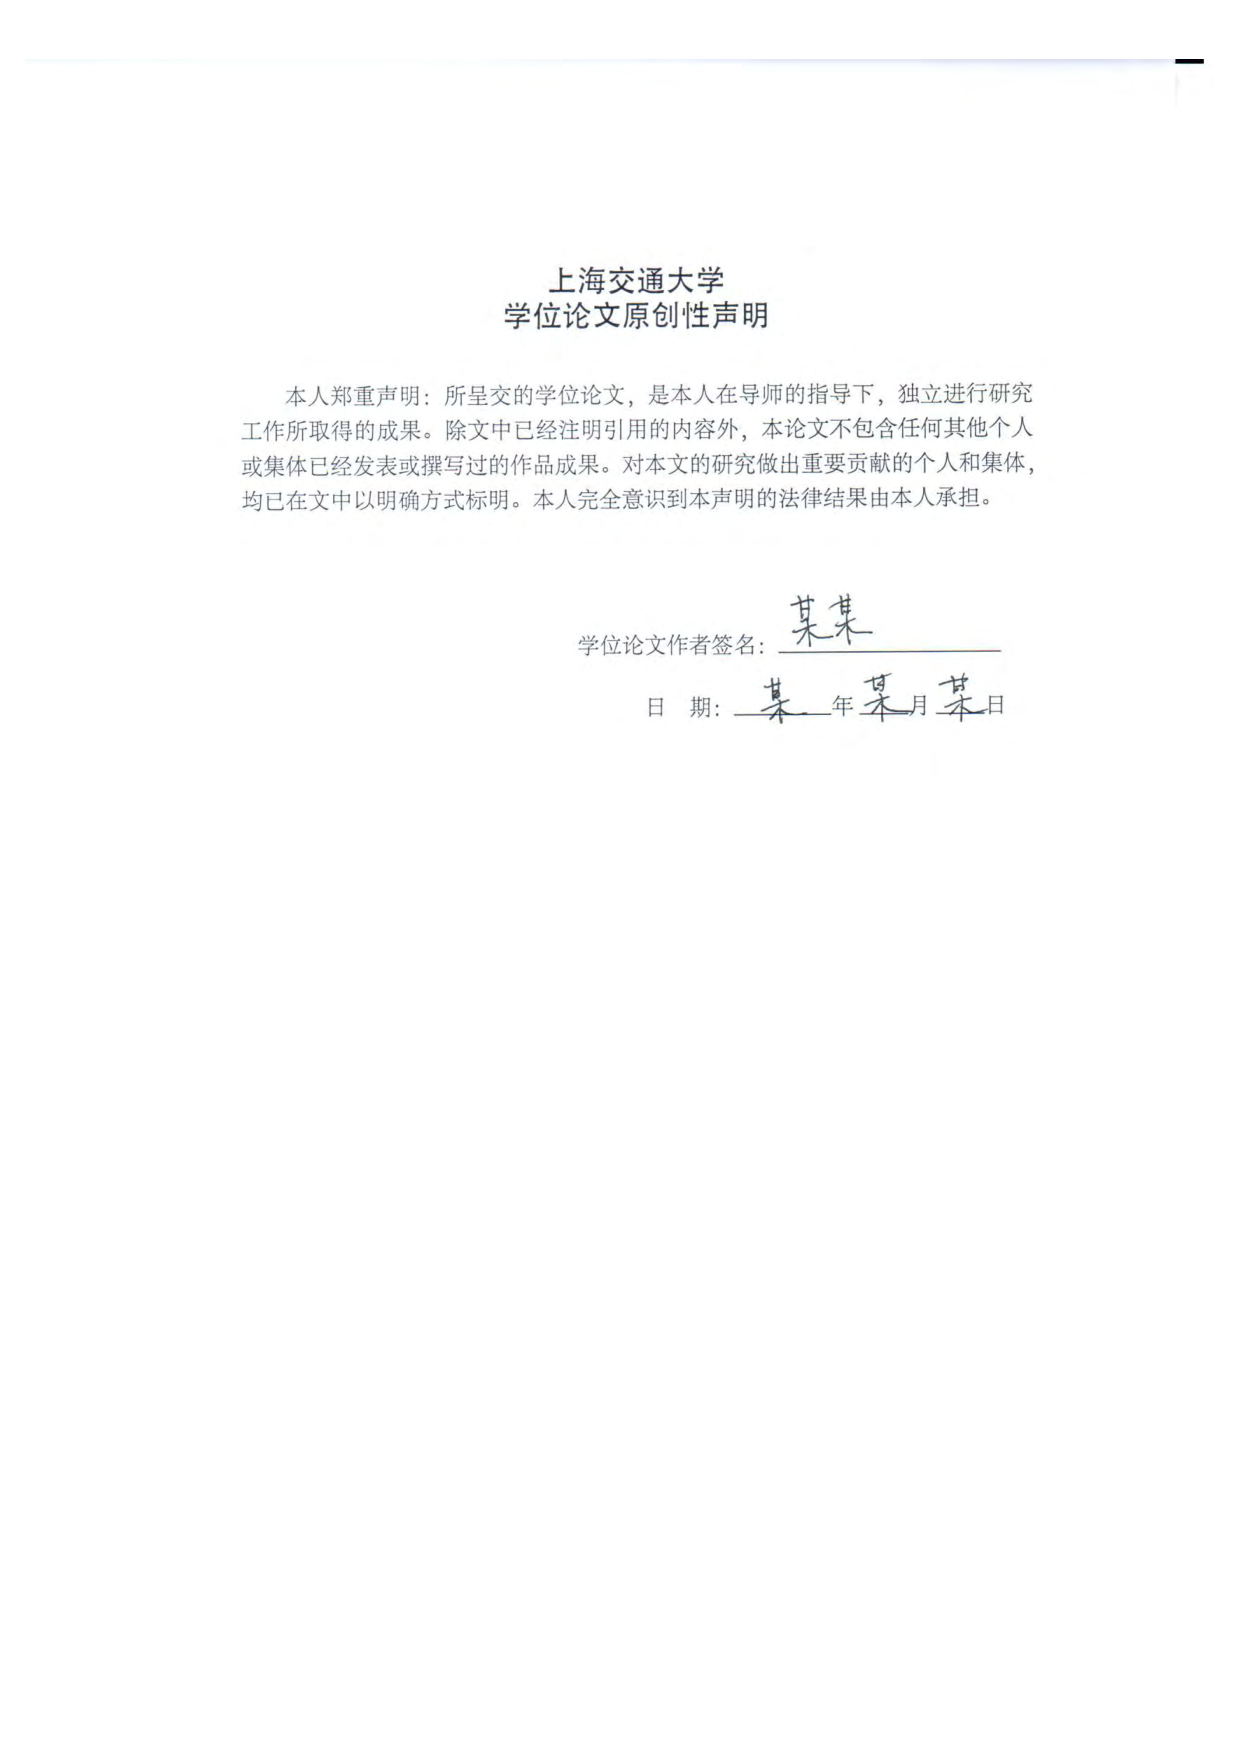
\includepdf{pdf/original.pdf}
	\cleardoublepage
	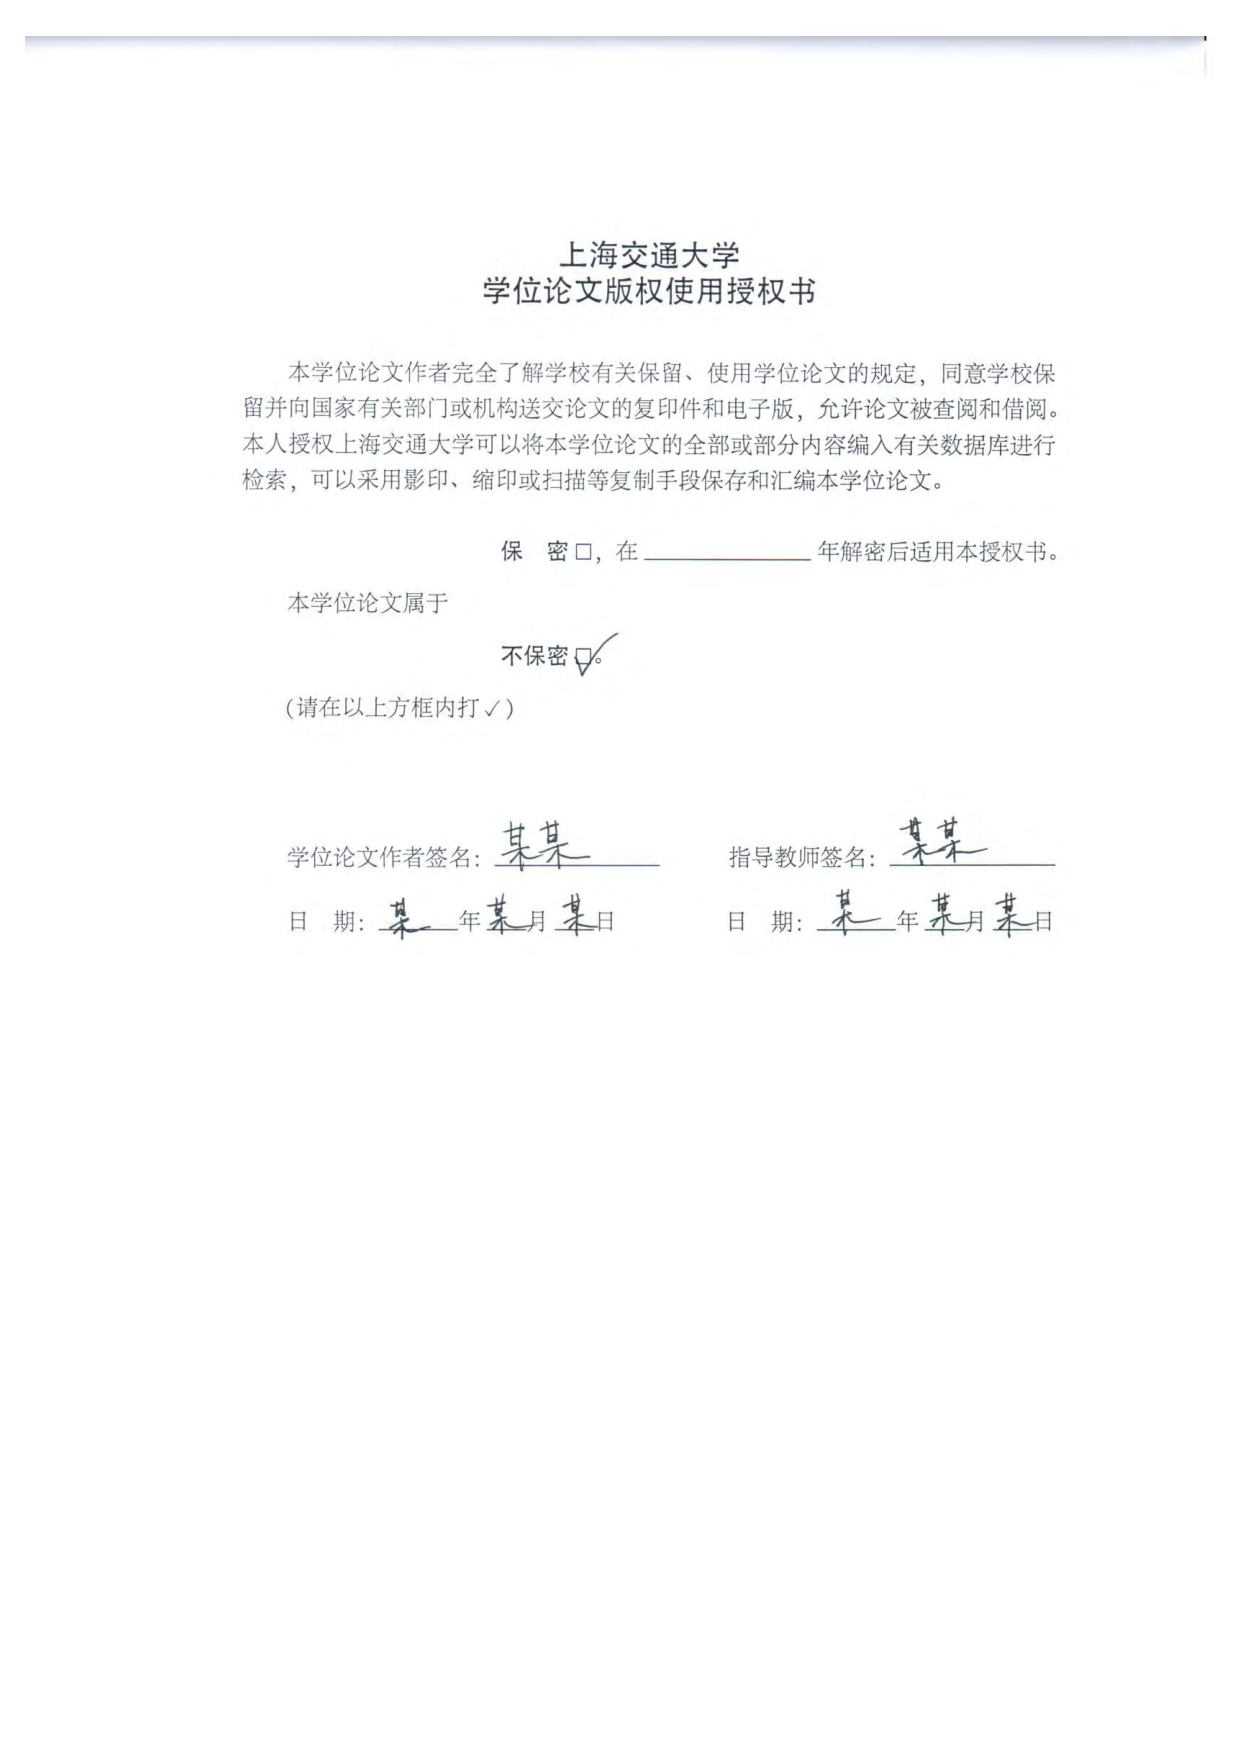
\includepdf{pdf/authorization.pdf}
	\cleardoublepage
\else
\ifsjtu@review\relax
% exclude the original claim and authorization
\else
	\makeDeclareOriginal
	\makeDeclareAuthorization
\fi
\fi
\makeatother


\frontmatter 	% 使用罗马数字对前言编号

%% 摘要
\pagestyle{main}
%# -*- coding: utf-8-unix -*-
%%==================================================
%% abstract.tex for SJTU Master Thesis
%%==================================================

\begin{abstract}

\keywords{\large 分布式存储 \quad 混合存储 \quad 负载均衡}
\end{abstract}

\begin{englishabstract}

\englishkeywords{\large Distribued Storage, Hybrid Storage, Load Balance}
\end{englishabstract}



%% 目录、插图目录、表格目录
\tableofcontents
% \listoffigures
% \addcontentsline{toc}{chapter}{\listfigurename} %将插图目录加入全文目录
% \listoftables
% \addcontentsline{toc}{chapter}{\listtablename}  %将表格目录加入全文目录
% \listofalgorithms
% \addcontentsline{toc}{chapter}{算法索引}        %将算法目录加入全文目录

\mainmatter	% 使用阿拉伯数字对正文编号

%% 正文内容
\pagestyle{main}
%# -*- coding: utf-8-unix -*-
%%==================================================
%% chapter01.tex for SJTU Master Thesis
%%==================================================

%\bibliographystyle{sjtu2}%[此处用于每章都生产参考文献]
\chapter{绪论}
\label{chap:intro}

\section{研究背景}
随着互联网行业的发展,如今的互联网正处于一个信息爆炸的时代。面对信息爆炸的互联网,对信息的存储和处理也就产生了海量的数据。
因此,传统的数据中心在性能、成本、安全和能耗上遇到了越来越多的挑战。为了应对海量数据带来的挑战,国内外一些大型IT公司都建立了各自的云系统和解决方案,
如亚马逊的AWS、微软的Azure、阿里巴巴的阿里云、百度的百度云等等。

为了高可用性和节约资源,IaaS(Infrastructure as a Service)云常常被用来部署大数据分析和其他各种类型的应用。 IaaS是以体系架构为基础的服务,
这些服务包括服务器、存储和网络硬件的提供。可是,如果以物理机的方式提供这些计算资源,那么成本将难以估计并且会造成大量资源的浪费。取而代之,现在的云提供商
选择以虚拟化技术来代替物理设备,这样充分降低了成本并且提升了可用性和可扩展性。在IaaS云,云提供商通过虚拟机监控程序虚拟化一台物理机,这样的虚拟化技术让
一台物理机运行多台虚拟机成为可能\cite{feng2014price}。因此,虚拟机被认为构建IaaS云的基础,而虚拟机常常是基于虚拟机磁盘镜像(VMDI)构建的。传统的云
存储解决方案,如NAS(Network Attached Storage)越来越难以适应大量的云存储需求,考虑到NAS的扩展性低、对非结构化数据没有优化的特点,用NAS存储虚拟机
磁盘镜像则毫无优势。相较于传统的NAS存储,对象存储由于其高扩展性可以更好地适应现在的大规模云存储。对象存储可以让云提供商轻松地扩大存储规模,并且它通过
备份数据副本的方式保证了存储的高可用性,更加重要的是对象存储允许存储大规模的非结构化的数据。对象存储是以对象为粒度管理数据,与之相对应的就是文件系统存储和块存储。
对象存储的一个重要设计原则就是抽象底层存储,使得底层存储于上层应用分离开来。对象包含了额外的描述性信息和属性,这样可以让对象可以被快速地索引和查找
现在一些云服务提供商,如亚马逊(AWS S3),微软(Microsoft Azure),还有一些开源项目如,OpenStack(Swift)、Ceph和OpenIO等等都是基于对象存储的。

对于存储介质方面,目前的主流存储介质包括了半导体存储和磁性磁性存储两大种类。对于半导体存储,其早在2006年笔记本和个人PC厂家就开始使用的SSD逐渐替代更多传统的磁体存储器HDD。
与传统机械硬盘HDD相比,SSD访问更加快速、可靠、低能效,但也更昂贵。在大量实验比较下,SSD的随机访问时间一般少于1ms,而HDD的随机访问时间则是在2.9至12ms之间,因此SSD的随
机访问速度是HDD的10倍以上\cite{kasavajhala2011solid}。纵然,SDD在性能、能耗等方面相较于HDD有较大的优势,但是由于其高昂的价格与存储空间比如传统硬盘仍有较大差距。
一个SATA WCD SSD的存储成本是1.375美元/GB,一个SATA WCD HDD的存储成本是0.068美元/GB。为了充分利用SSD的性能潜力,现在关于混合存储的研究主要是将SSD作为前端存储(缓存)
或作为主存。如果将SSD作为存储缓存则必须面对两个主要问题:缓存和主存之间的一致性问题以及SSD的容量浪费问题。那么,如果将SSD作为主存,那么混合存储的关键性问题在于把哪些对象放置于SSD。

实验室学长在本文开始之前已经有了关于混合存储的的研究,分别是WHOBBS\cite{lingxuan2015whobbs}和MOBBS\cite{ma2014mobbs},它们基于对象存储为虚拟机提供混合存储的块服务。
它们都在Ceph\cite{weil2006ceph}的基础上,构建了一套完整的混合存储系统。它们最根本的思路是,将过热的数据放置在SSD上,反之将较冷的数据放置在HDD上。这两个系统都是通过数据
对象的数据流监控,数据流包括数据对象的大小、特定的访问类型等等信息。它们将这些数据流信息进行处理之后得到每个对象的热度值,然后根据每个对象的热度值制定一个合适的迁移策略,使得
每一个对象对象都放置在合适的存储设备上。WHOBBS是MOBBS的升级版本。MOBBS将对数据流的监控分析模块和虚拟机管理器都放在客户端节点,因为监控分析模块会占用客户端节点的计算资源,这
样势必会直接影响到虚拟机管理器和虚拟机的运行效率。WHOBBS在MOBBS的基础上修正了这个问题,它把监控分析模块分离出来,放在一个独立的节点上去运行,它叫做Monitor。这样就是支持多个
客户端节点同时运行,并且把MOBBS存在的性能隐患也完全消除。WHOBBS相较于MOBBS虽然可以很高效,但是考虑到WHOBBS是单监控节点架构,那么当客户端的数量增加起来之后,监控节点的计算压
力也会随之增长。这样势必还是会影响到整个系统的性能。不仅如此,因为WHOBBS的Monitor成为了整个系统的关键性节点,那么Monitor节点一旦宕机,整个系统都不能正确运行。

\section{研究目标和内容}
本课题的目标是,第一,优化现存分布式混合存储中的监控节点,创建多个监控节点,实现监控节点的分布式,从而保证分布式混合存储系统的高可用性;第二,根据用户行为,对存储内容的访问情况,动态调整存储策略,下层的混合存储实现对用户透明;
第三,混合存储的关注点不再具象到HDD/SDD这两种存储介质,而是探索不同存储介质的特性,动态适应混合存储系统。

\begin{itemize}[noitemsep,topsep=0pt,parsep=10pt,partopsep=10pt]
	\item 分布拓扑结构监控器:由于在现存的分布式混合存储系统中,都存在一个监控节点,但是由于只有一个监控节点,这样使得管理节点往往成为性能的瓶颈。为了解决这个问题,需要创建多个管理节点,也就是对管理节点分布式。
	\item 分布式全局热均衡:本课题的第一个目标就是创建多个监控节点,实现监控节点的分布式。那么这将带来一个问题,每个监控节点分管不同的混合存储节点,因此监控节点可以较好得保证各自分管的混合存储节点内部的热均衡,但是这只是局部的热均衡并不是全局的。全局热均衡需要提出适当的算法、合适的策略、完善的数据迁移方法。	
	\item 面向多存储介质的数据放置方法:不同存储介质在对不同类型或频率的IO请求都会存在性能上的差异。所以要通过实验来确定存储介质的特性,并根据其性能上的特性设计数据放置方法,然后将计算出的放置方法应用到混合存储的数据迁移策略中。
\end{itemize}

\section{研究意义}

\section{论文组织结构}
本文正文包含六章,本章为绪论,首先系统性地介绍并分析了本课题的研究背景和研究意义,在此基础上提出了本课题的研究内容和目标。其他章节的内容组织如下:

第\ref{chap:relatedwork}章介绍了和本课题有关的国内外研究现状。该章节从本课题所涉及的研究内容出发,调研并分析了与之相关的现有的国内外研究成果与不足,并提出了可以进一步研究和改进之处。

第\ref{chap:systemdesign}章介绍了本课题提出的移动边缘计算的体系架构设计。该章节首先从整体上介绍了移动边缘计算的体系架构,之后对架构中的具体模块进行了详细的分析和设计。

第\ref{chap:systemimpl}章介绍了系统实现。该章节分别介绍了移动边缘计算的体系架构各个模块的实现、上下文感知的计算服务动态感知方法的实现以及云-端负载平衡的计算迁移机制的实现。

第\ref{chap:experiment}章介绍了系统实验与验证。该章节详细地介绍了为验证本课题所提出的移动边缘计算的体系架构以及云-端负载平衡的计算迁移机制所进行的实验,并针对实验结果给出了详细的分析。

第\ref{chap:summary}章为总结与展望。该章节总结了本课题的主要研究工作与贡献,并在此基础之上给出了今后的研究方向。
%# -*- coding: utf-8-unix -*-
%%==================================================
%% chapter01.tex for SJTU Master Thesis
%%==================================================

%\bibliographystyle{sjtu2}%[此处用于每章都生产参考文献]
\chapter{国内外研究现状}
\label{chap:relatedwork}
随着云计算的高速发展,每天在互联网中都会产生海量的数据。分布式存储作为云计算的基础,近些年有大量的关于分布式存储的研究。
以下将通过:分布式存储及对象存储、混合存储的应用以及分布式存储负载均衡等几个方面来进行国内外研究现状的综述。

\section{分布式存储及对象存储}
分布式存储作为云计算的基础,谷歌在2003年提出的GFS\cite{ghemawat2003google}是在分布式系统领域具有划时代意义的论文,它的提出了如何采用
廉价的商用计算机集群构建分布式文件系统,论文中提出的控制与业务相分离、将容错的任务交由文件系统来完成、多副本机制等等,这些概念大多都变成了
之后分布式存储系统设计研究的金科玉律。在随后的Apache的HDFS\cite{shvachko2010hadoop},在一些设计上与GFS高度一致,它提供了一个高度容错的分
布式文件系统,能够提供高吞吐量的数据访问。

对象存储的概念在上个世界90年代就应该在研究社区中出现,但是在当时由于云计算还没有广泛流行,所以对象存储也没有被广泛运用。对象存储,是将对象作为单位管理数据,与之对应的
文件存储则是以文件系统结构为基础,而块存储则是以块为单位管理数据。\citen{factor2005object}介绍了对象存储发展的几个阶段,首先是由TIO OSD协议作为第一阶段的标准,
第二阶段则是iSCI。Ceph作为当今非常流行并且成熟的分布式对象存储,已经集成到了Linux内核中。Ceph是一个基于对象存储的PB级分布式文件系统,
拥有极佳的可靠性和可扩展性。根据配置的不同,Ceph可以分别提供上述的块存储、文件存储和对象存储三种服务,但是所有的服务均基于一个叫Rados的对象存储系统。

\section{混合存储的应用}
SSD的读写性能、能耗等各个方面较于传统的HDD有较大的优势,因此近些年来SSD被越来越多的用于计算机存储领域。\citen{kasavajhala2011solid}中揭示了SSD和HDD性能上的差距,
并且建议用户通过价格和性能的比率来选择合适的存储设备,对于不同的数据流SSD和HDD在性能上的表现也有一定的差别。对于顺序数据流,SSD在性能上的提升相较于其高昂的
价格就并没有太多的优势,而对于随机数据流SSD对于读写性能的提升十分显著。因此考虑到SSD高昂的价格,以及其在特定数据流表现的性能差异,将SSD与HDD作为存
储设备混合使用将会是一个研究的重点。

对于关于SSD/HDD混合存储的研究主要分为两类,一类是考虑到SSD相较于HDD具有节能、高效的特性,将其用作存储缓存;另一类是考虑到SSD较高的读写性能、非易失性以及拥有大容量,
将SSD作为主要二级存储。以下将从这两类介绍SSD在混合存储中的应用。

在\citen{wan2014ssd}中,作者提出了一个混合式的对象放置和移动架构,以及适应性学习算法来识别数据对象的访问热度。该论文中,混合式架构通过将数据对象在慢速的HDD和快速的SSD间相互移动来适应
数据对象访问热度的动态变化,同时数据对象的放置及移动规则也可以满足用户对它们I/O操作的需求。基于以上的目标,论文提出了一个基于马尔科夫链的识别模型来预测数据对象在外来一段
时间的访问频率,这个识别模型是以对象的访问模式为训练集训练马尔科夫链模型,一旦的得到预测结果就开始在HDD和SSD间迁移数据。为了适应用户自定义的放置规则,论文提出了一个数据放
置引擎,以用户的放置需求作为输入产生合适的解决方法。\citen{wan2014ssd}的核心思想就是,作者将SSD和HDD的混合存储用到了高性能计算领域(HPC),因为是它基于预测的思想,所以可以在整个系统数
据发生变化之前就将数据进行迁移,这样大大提高了整个系统的IO性能。

\citen{li2015trade}将目光放在了对SSD/HDD混合存储在性能、耗能和寿命问题做出了研究。\citen{li2015trade}设计并实现了一个多用的混合存储驱动,它实现的混合存储系统包含两个模式——分层存储模式和缓存模式,
这两个模式分别将SSD用作存放热点数据的主存和用于存储热数据的缓存。该系统从混合虚拟设备接受数据访问请求,并将结果重定向给下层物理设备。而\citen{li2015trade}在区分冷热数据的方式与\citen{wan2014ssd}相
似,也就是将热的、访问频率高的数据放在SSD中,反之冷的、访问频率低的数据放在HDD中,当数据的冷热情况发生变化,再动态地将数据进行迁移。但是它把研究的重心放在了对性能、耗能以及寿命的权衡。它得出的结论是,
为了得到高性能,势必会导致能耗的增加;对于论文中,数据分块越大性能提升越大,同时会造成SSD寿命的快速衰减。\citen{wan2014ssd}和\citen{li2015trade}都分别研究了以SSD/HDD为主体的混合存储,并且研究的重
点都在于利用SSD在读写方面优异性能,将热点数据存储在SSD中,冷的数据存储在HDD中,再通过这一基本框架做进一步的研究。

而\citen{wan2017optimizing}的研究重点面向了更加特定的环境,即面向高性能计算环境下基于SSD突发缓存的研究。\citen{wan2017optimizing}的研究不仅限于SSD/HDD这两种局限的存储介质类型,而是更加抽象的存储分层,它以SSD作为突发缓存,
而底层存储是并行文件系统(PFS),突发缓存作为客户端与并行文件系统之间的缓存,常常要存储检查点(checkpoint),而检查点是需要频繁读写的,这样会造成SSD的寿命大幅缩短,并且由于高性能计算环境数据流往往是高速、大流量的,所以对作为突发缓存的硬件寿命
面临着极大的挑战。基于这个问题,\citen{wan2017optimizing}设计了一个适应性算法基于高性能计算环境下系统数据流的变化,动态的切换检查点的放置策略,这样既保证了系统的高效运行也大大延长了突发缓存的硬件寿命。

Apple公司在2012年发布了自己的混合存储设备Fusion Drive,并将其应用到Apple的各个产品中。Fusion Drive融合了HDD和SDD,系统会自动管理访问最频繁的应用程序、文件、照片或者其他数据来存储在SSD里,而将很少访问或使用的文件留在机械硬盘上。
\citen{chen2011hystor}为Apple开发Fusion Drive提供了思路。在\citen{chen2011hystor}中,作者设计并实现了一个高性能混合存储系统Hystor。作者在论文中提出了混合存储必须面对的三个问题,分别是1)高效地识别性能关键的数据快并充分利用
SSD的存储潜力;2) 为了精确地刻画数据访问模式必须高效地保存数据访问历史;3) 系统实现的过程中避免对现存操作系统内核的改变。\citen{chen2011hystor}实现的Hystor充分解决了上述的三个问题,它通过监控I/O自动地学习数据流访问模式并识别出
性能关键的数据块,只有带来最大性能收益的数据块才可以从HDD重映射到SSD中;其次,Hystor设计了一个高效的机制即数据块表(Block Table)去存储数据块访问的历史信息,这样可以为长期的优化提供资源;它是一个Linux的内核模块,只对内核做了很少的修改。
因此\citen{chen2011hystor}作为一个具有里程碑意义的论文,颠覆了以前仅仅利用SSD优秀读写性能而将SSD作为缓存的传统模式,而提出了将SSD和HDD混合做个主要存的新模式。

对于\citen{krish2014hats},它将混合存储用到了HDFS(Hadoop Distributed File System)中,由于原有的HDFS并不能用来处理多层存储,。HDFS认为所有底层存储组件都具有相同的I/O特性,这样会造成对资源的浪费和不高效实用。因此,在\citen{krish2014hats}中,
作者设计并实现了一个针对Hadoop的多层存储系统hatS,它在逻辑上把相同存储类型的节点分到同一个层,这样单独地管理各个存储层,hatS就能够捕捉分层信息并充分利用这些信息从而达到高的I/O性能 。与HDFS不同的是hatS使用分层感知的方法在不同之间复制数据,这样使得
高性能存储设备可以高效地处理更加处理大量I/O请求。hatS的实际做法是利用Hadoop的多数据备份的规则,并结合存储分层,让尽量多的I/O请求作用到性能高的节点上,从而提升整个系统的吞吐能力。

\citen{ma2014mobbs}\citen{lingxuan2015whobbs}两篇论文,将混合存储和当今非常流行的对象存储系统Ceph相结合,\citen{ma2014mobbs}设计并实现了基于Ceph的混合存储系统WHOBBS。由于原始的Ceph系统并没有对底层存储介质的类型给予优化,它是根据CRUS
H算法\cite{weil2006crush}静态地设置osd权值,根据权值放置数据,这个过程是静态的,并不能使用数据访问热度的动态变化。因此WHOBBS动态监测每一个数据对象,并且保存数据对象的历史访问记录,根据用户自定义算法来指定迁移策略,即SSD与HDD之间的迁移策略。在设
计迁移策略之前,\citen{lingxuan2015whobbs}做了大量实验验证SSD与HDD在Ceph不同数据流下的性能,并根据实验结果指定合理的数据对象迁移策略。

综上所述,现今关于混合存储的研究大多都着眼于利用SSD优秀的存储性能以及低能耗等特点,但是由于SSD高昂的价格、有限的寿命以及在部分数据流方面表现的差异,所以现在仍用很多数据存储公司权衡这方面的利弊,选择了混合存储架构。如现在的Apple FusionDrive、
Microsoft公司的Ready Drive、西部数据公司的SSHD等等。而这些产品大多都是面向单机存储的,它们并没有充分应用到分布式存储的环境中,正如\citen{krish2014hats}所说,现在的大部分的分布式计算框架对待底层存储都没有根据存储的类型来进行优化。

\section{分布式存储负载均衡}
在大规模云计算环境中,负载均衡技术通过保证每一个计算资源可以获得公平的计算请求,达到了用户满意度,同时提高了资源利用率。合适的负载均衡目技术为的就是减小资源竞争、保证可扩展性、避免性能瓶颈等等。

Paiva J.等人在2015年提出了AutoPlacer\cite{paiva2015uto},它面向现今最流行的键值存储提供数据放置策略,AutoPlacer的自调节数据放置策略可以较好地达到负载均衡目标。AutoPlacer使用了一个轻量级的分布式优化算法
,这个算法不断迭代,在每一次迭代中它以一种去中心化的方法优化前K个热点数据的放置。热点数据实际上产生最多远程操作的数据对象。为了识别出热点数据,并且不会有对整个系统的性能带来太大的影响,AutoPlacer
选用了一种全新流分析算法来追踪数据流(data stream)中前K个最常被访问数据对象。AutoPlacer不仅支持细粒度的数据放置,还使用了全新的概率数据结构PAA来保证单跳路由的延迟最小。


\citen{zhang2015skewly}提出了一个全新的想法,它使用倾斜的复制策略来构建节能存储集群。它提出的数据复制策略实际是基于数据访问行为的。这个策略仅仅复制访问热点数据,而这些热点数据根据80/20原则(80\%
的数据访问往往只访问20\%存储空间的数据)恰恰只是整个数据齐群20\%的数据量。因此,可以将集群分为热节点集和冷节点集。热节点存储较少数量的数据副本,并且常常处于活跃状态来保证整个系统的QoS
。冷节点则与之相反,它存储数量较大且访问频率较小的冷数据,并且这些存储节点被通过一定的方式(CPU降频、磁盘降低转速)来进入节点模式。作者在论文中通过模式实验中验证了自己的观点,其所提出的系
统不仅可以保证低能耗也可以保证整个系统的性能不受到影响。

Soni G.等人另辟蹊径提出了全新的云数据中心的负载均衡方法\cite{soni2014novel}。这个负载均衡方法面向云数据中心的虚拟机数据流。每一个来自用户的请求都从数据中心控制器发起,数据中心控制器遍历中心负载均衡器,通过遍历结果来分配请求。
中心负载均衡器会维护一个包含id、虚拟机状态以及虚拟机优先级的数据表。中心负载均衡器分析数据表并且找到最高优先级的虚拟机,然后检查其状态,如果它的处于可用的状态则返回虚拟机id给数据中心控制器。最终,数据中心控制器
将会把某个数据请求分配给特定的虚拟机。作者通过实验验证了中心负载均衡方法的可行性。

Deng Y.等人提出的负载均衡技术\cite{deng2014dynamic}进行了创新,他们利用了物理学的热扩散原理来处理分布式虚拟环境(DVE)的负载均衡问题。在论文中,作者使用了一种混合式的负载均衡策略,也就是将全局负载均衡和局部负载均衡相融合。全局负载均衡指的是,
存在一个中心节点来管理所有服务器的负载情况,它从各个服务器收集负载数据,并制定负载策略,这样做的优点就是可以准确地实现负载均衡,但是计算量较大,需要额外的计算资源。与全局负载均衡相反,局部负载均衡则不存在中心节点,每个服务器通
过其邻接的服务器负载数据来制定自己的负载均衡策略,这样做的优点在于计算量较小,但是负载的结果不并准确。在\citen{deng2014dynamic}中,作者使用了热扩散原理,即高温区域的热量会向低温区域扩散,来处理负载均衡问题,并且将热扩散原理与全局负载均衡和局部负
载均衡相结合,提出了局部扩散和全局扩散。对于热扩散在负载均衡中的应用,高度概括为,过热服务器将自己的部分数据流交给邻接较冷的服务器去处理。作者通过大量的实验和数学证明验证了基于热扩散的负载均衡技术的高效性。

综上所述,现在已经有许多在分布式系统负载均衡方面的研究,但是可以发现一点,就是这些\citen{paiva2015uto}\citen{zhang2015skewly}\citen{deng2014dynamic}关于负载均衡的研究都是相对静态的,并且大多是关于数据放置如何达到负载均衡,
并没有考虑计算节点过热时如何动态均衡计算任务。

\section{本章小结}
本章通过分布式存储和对象存储、混合存储和分布式存储负载均衡,这三个方面介绍了与本课题相关的国内外研究现状。分布式存储和对象存储介绍了,现在主流的分布式存储框架以及Ceph等对象存储系统,并叙述了这些系统
在特点及应用场景。混合存储部分,从SSD和HDD的性能差距着手阐述了混合存储的必要性和意义,之后分别介绍了国外关于混合存储的研究。混合存储的主要研究还是主要面向于将SSD运用为主存,或是将SSD运用为缓存。但是现在
关于混合存储的研究大部分还是面向单机存储的,分布式存储的应用相对较少。分布式负载均衡部分,介绍了多种分布式存储负载均衡的解决方案,但是可以清楚地看到,大部分解决方案都是满足静态的负载均衡,而对于运行时(动态)的负载均衡
都没有涉及。
%# -*- coding: utf-8-unix -*-
%%==================================================
%% chapter01.tex for SJTU Master Thesis
%%==================================================

%\bibliographystyle{sjtu2}%[此处用于每章都生产参考文献]
\chapter{系统设计}
\label{chap:systemdesign}
DOBBS是为了适应大规模IaaS云的底层存储,利用对象存储对非结构化数据VMDI进行大量优化,并且在WHOBBS的基础上解决了其性能缺陷。本章我将介绍DOBBS的
系统架构设计以及各模块设计。

\section{DOBBS架构介绍}
所谓混合存储系统,就是将SSD与HDD共同组合而成的存储系统。DOBBS的系统设计是基于Ceph实现的,而Ceph的文件实际是存储在对象存储设备中的(Objects 
Storage Device)。为了提升DOBBS系统的高扩展性,我们借用了Ceph存储池(Storage Pool)的概念。存储池实际是部分对象存储设备的逻辑集合,一个存储池
可以包含多个对象存储设备,而对象存储设备是挂载在物理存储介质上的。因此对于DOBBS,我们有两种类型的对象存储设备,分别是SSD对象存储设备和HDD对象存储设备。
之后,我们将部分SSD对象存储设备和部分HDD对象存储设备共同组织成一个混合存储池(Hybrid Storage Pool)。混合存储池中的对象存储设备是可以由用户配置的,
通过这样的组织,DOBBS的底层存储集群可以简单高效地扩展。一般性的,每个混合存储池都至少包括一个SSD对象存储设备和至少一个HDD对象存储设备。


\begin{figure}[!htp]
    \centering
    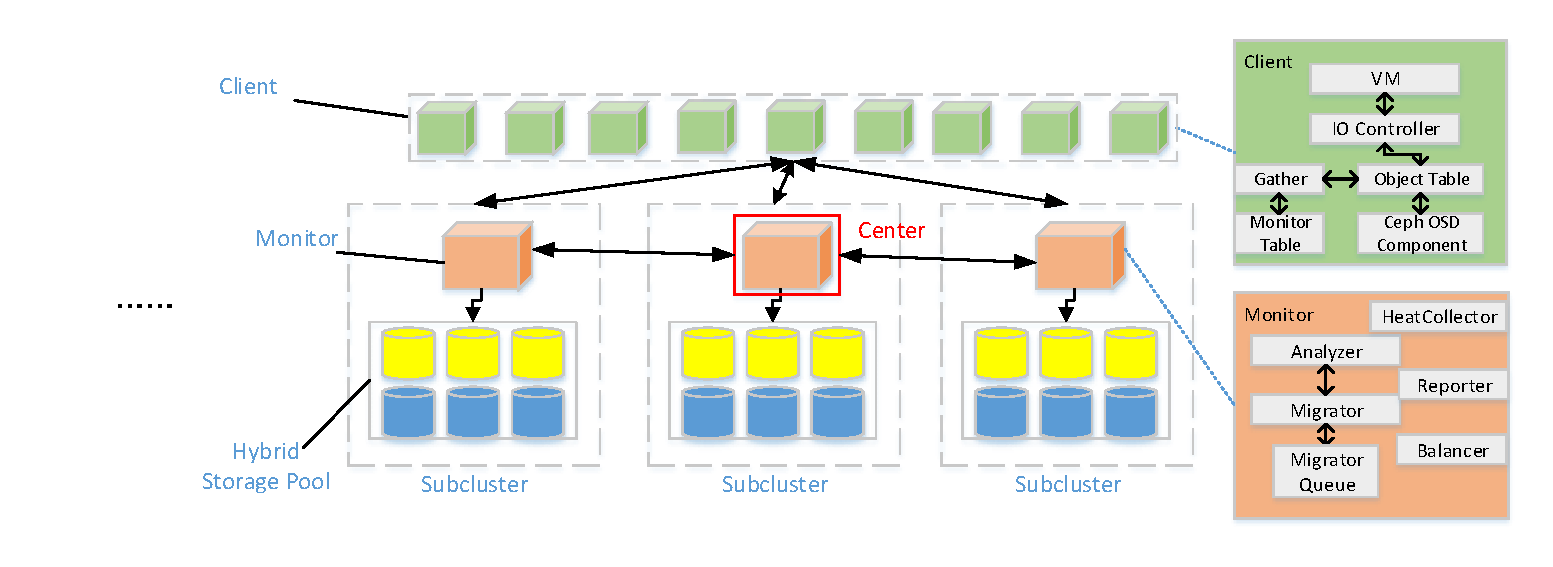
\includegraphics[width=16cm]{example/Arch.pdf}
    \bicaption[fig:arch]{DOBBS系统架构图}{DOBBS系统架构图}{Fig}{Architecture of DOBBS}
   \end{figure}


如图\ref{fig:arch}所示为DOBBS的系统架构图。DOBBS的架构大致可以分为两层,一层是存储集群也就是混合存储池,一层是监控器(Monitor)。DOBBS包含大量
的混合存储池以及监控器。存储集群正如上文所说的,它是有大量的混合存储池组成的。为了系统的高可靠性和高性能,我们将一个监控器和一个混合存储池绑定在一起,组成一个子
集群(subcluster)。之所以要划分成子集群是因为多个Monitor如果同时管理所有的混合存储池势必会造成管理的混乱,并大大降低系统的可扩展性。引入子集群则是可以充分
提升系统的可扩展性,并使整个系统易于管理。监控器在DOBBS则是起到至关重要的作用,它的作用包括监控虚拟机的数据流信息并生成合适的迁移策略,还有检测其所在子集群的热度并向中心节点(Center)
汇报,最终执行全局热均衡迁移指令。在DOBBS中,子集群仅仅只是逻辑上的概念,虚拟机VMDI则被均匀的分布在各个子集群的混合存储池中。监控器所监控的数据流信息也仅仅是其所在
子集群对应数据的数据流信息。客户端(Client)则是虚拟机管理器(VMM)所运行的机器,它们是DOBBS所提供服务的对象,客户端在接入DOBBS之后,与底层存储系统交互并进行数
据读写。中心节点则是DOBBS的监控器集群的大脑,它的主要作用是收集每个子集群的热度信息,并保证整个系统的热均衡。关于整个系统的热均衡,在本章后续章节将会叙述。

为了系统的高内聚低耦合,我们将系统分为多个模块,模块间互相依赖并支持高效扩展。在客户端上,如果让虚拟机管理器直接访问Ceph的块存储,那么它只需要调用Ceph提供的
OSD Component接口即可,但是为了获得虚拟机的数据流信息我们VM与Ceph存储设备的交互中间增加了一层DOBBS监控组件。因为Ceph是对象存储系统,所以虚拟机访问的粒度都是
一个个对象。如图\ref{fig:arch}所示,IO Controller负责截取VM的访问请求,然后通过查询Object Table来知道对象是在哪个OSD上,这是因为在数据迁移的过程中对象被频繁迁移,
而Ceph访问对象是通过对象ID和OSD共同组合访问,因此需要一个数据结构在存储对象ID和OSD ID的映射。Gather模块类似于一个计数器,它会记录每一个单位时间间隔内的
对象的访问次数、访问类型等信息,在记录之后再定时发送给Monitor。Monitor Table则是用来维护OSD ID和子集群ID映射的,因为在DOBBS在保证整个系统热均衡的过程中需要对OSD上的数据进行跨子集群迁移,所以
可能会导致某个OSD的位置发生了改变。最终,Ceph根据VM请求的对象ID和OSD ID来和底层存储进行交互。

Monitor主要有六个模块。Analyzer模块是Monitor的大脑,它负责接收客户端传送过来的虚拟机数据流信息,然后根据内置算法来生成合适的对象迁移命令,命令产生后将迁移命令传递给
Migrator模块执行。Migrator得到迁移指令之后,进行后续的上锁等等操作,然后再将最终的指令缓存在Migrator Queue中,这个队列的长度是DOBBS所支持的最大迁移数量,这个数量
当然也是可配置的。在Monitor上还有三个独立的模块,Reporter、HeatCollector和Blancer,他们都是用来负责系统热均衡的。

DOBBS提出了两个重要的概念,局部热均衡和全局热均衡。对于局部热均衡,我们数据对象分为两类,热对象和冷对象。所谓热对象是指的那些访问频率高,短时间内会被多次访问的对象。相反,
冷对象则是指那些访问频率并不高的对象。为了充分利用SSD的性能优势,我们将热对象都放置于SSD上而将冷对象都放置于HDD上,然后动态地监测数据对象的冷热变化来在SSD和HDD之间迁移对象。
局部热均衡只是针对每个子集群内部的局部热均衡,因此每个Monitor只能保证所在子集群的局部热均衡。如果将存储集群和Monitor分割成多个子集群,那么极有可能在
某个时刻某个虚拟机产生了非常大量的VMDI请求,这样某个子集群会遭受大量的读写请求,数据也会频繁地在SSD和HDD间迁移,这个子集群的效率将会受到极大影响。提出全局热均衡的概念就是为了
消除上述情况带来的性能波动。全局热均衡针对的粒度是OSD级别的,它会动态监测每个子集群的热度,然后做出迁移指令,有别于局部热均衡的迁移,全局热均衡的迁移是将OSD的数据进行迁移而不是
在OSD进行数据对象的迁移。

\section{局部热均衡}



%# -*- coding: utf-8-unix -*-
%%==================================================
%% chapter01.tex for SJTU Master Thesis
%%==================================================

%\bibliographystyle{sjtu2}%[此处用于每章都生产参考文献]
\chapter{系统实现}
\label{chap:systemimpl}
本章在上一章的基础上,介绍DOBBS在实现过程中所用到技术以及各个模块的具体实现情况。

\section{实验工具和平台}
\subsection{Ceph}
Ceph是一个免费开源的存储平台,它将对象存储实现在一个分布式计算机集群内,并且为对象级、文件级和块级存储提供了接口。Ceph主要针对完全分布式操作,没有单点故障,可以扩展到exabyte级别,并且有非常高的可用性。
Ceph的软件库为客户端应用程序提供了对RADOS基于对象的存储系统的直接访问,同时提供一些高级功能,包括RADOS Block Device(RBD),RADOS Gateway(RGW)和Ceph File System(Ceph FS)。

Ceph的对象存储系统允许用户将Ceph安装为精简配置的块设备。 当应用程序使用块设备将数据写入Ceph时,Ceph会自动在整个群集中对数据进行分条和复制。 Ceph的RADOS Block Device(RBD)还集成了基于内核的虚拟机(KVM)
Ceph的块设备可以被虚拟化,为虚拟机提供块设备服务在一些主流的虚拟化平台都使用Ceph,例如Apache CloudStack、Openstack和OpenNebula\cite{milojivcic2011opennebula}等等。

DOBBS在Ceph的基础上进行修改是因为,Ceph是对象存储系统,当虚拟机在Ceph存储集群创建VMDI之后,Ceph会默认地把它分割成等大小的对象,而DOBBS需要动态监测虚拟机VMDI的数据流,那么如果VMDI已经被等大小分割那么我们就可以直接地
监测Ceph对象而不是整个VMDI数据块,这样把监测和迁移的粒度放到比较小,帮助我们快速准确的迁移数据。还有一点就是,Ceph与虚拟化的结合很充分,所以不需要我们特别地为Ceph进行额外的修改。

\subsection{QEMU}
QEMU\cite{bellard2005qemu}是快速模拟器(Quick Emulator)的缩写,它是一个免费的开源托管型虚拟机管理程序,可执行硬件虚拟化。QEMU是托管的虚拟机监视器:它通过动态二进制转换模拟CPU,并提供一组设备模型,使其能够运行各种未修改的客户机操作系统。 
它也可以与KVM\cite{kivity2007kvm}一起使用,以接近本机的速度运行虚拟机。 QEMU还可以为用户级进程执行CPU仿真,允许为一个体系结构编译的应用程序在另一个体系结构上运行。QEMU的优势在于,它足够轻量级并且已经被合并入Linux内核。而在本论文中选用
QEMU作为虚拟机管理程序主要有两个原因,一是因为QEMU是开源软件我们可以直接对其源代码进行侵入式修改,二是QEMU已经有了针对于Ceph的虚拟块存储服务。

\subsection{Apache Thrift}
Thrift是一个RPC(Remote Procedure Call)框架。Thrift是一种接口定义语言和二进制通信协议,用于定义和创建多种语言的服务。它被用作远程过程调用(RPC)框架,并在Facebook上为“可扩展的跨语言服务开发”而开发。Thrift的使用
非常方便,用户只需要写一个自定义语言的文件用于定义接口和部分数据结构,之后主要输入Thrift的指令便可以生成对应语言的服务器/客户端文件。在DOBBS的实现中,我们用Thrift作为跨服务器远程过程调用的工具,我们只需要编写Thrift自己定义
语言的接口语言,并可以在各个服务器上使用,十分便捷。
\begin{lstlisting}[language={C++}, caption={Thrift 接口定义示意}, label={code:thrift}]
    struct ObjInfo {
      1:string m_eid,
      2:i32 m_osd,
      3:double m_rio,
      4:double m_wio,
    }
    struct MonitorMetadata{
        1:string m_eid;
        2:i32 m_osd;
        3:double m_weight;
        4:string m_ip;
    }
    
    service MonitorService {
        void finish_lock(1:string eid),
        void report_client_info(1:ObjInfo ci),
        void finish_migration(1:string eid),
        void begin_heat_diffusion(1:string to_ip),
        list<MonitorMetadata> exchange_metadata(1:i32 pool_id, 2:list<MonitorMetadata> monitor_extents),
        bool get_monitor_lock(),
        void release_monitor_lock(),
    }
\end{lstlisting}

如代码\ref{code:thrift}所示为Thrift接口定义代码,该代码表示DOBBS的Monitor模块的对外提供的接口。首先需要定义用于传输的数据结构,在Monitor中,我们需要收集从Client发送的对象
数据流信息,所以接口定义中我们用ObjInf来表示。service代码块表示具体接口的接口名以及参数和返回值等等。在编写完接口定义文件之后,用户需要调用Thrift程序即可生成指定语言的代码,然后用户
将代码拷贝到需要调用接口的计算机上,即可完成RPC传输。

\section{系统模块实现}
如图\ref{fig:implmain}是系统模块结构图。从图中可以看到,DOBBS主要有四个组件,分别是客户端(Client)、监控器(Monitor)、OSD和中心控制器(Center)。
而我们的各个模块分布在了这些组件上。在本章系统实现部分我们不再用模块的概念来表述,图\ref{fig:implmain}的类则对应了上一章系统架构图中的各个模块。为了
直观显示DOBBS各个组件之间的关系,我们将Center独立出来作为一个组件描述,而实际场景中,Center是位于某个Monitor服务器上运行的。值得注意的是,图中的Ceph OSD Component
并不是DOBBS中的组件而是Ceph系统所提供的访问数据对象的接口。

\begin{figure}[!htp]
    \centering
    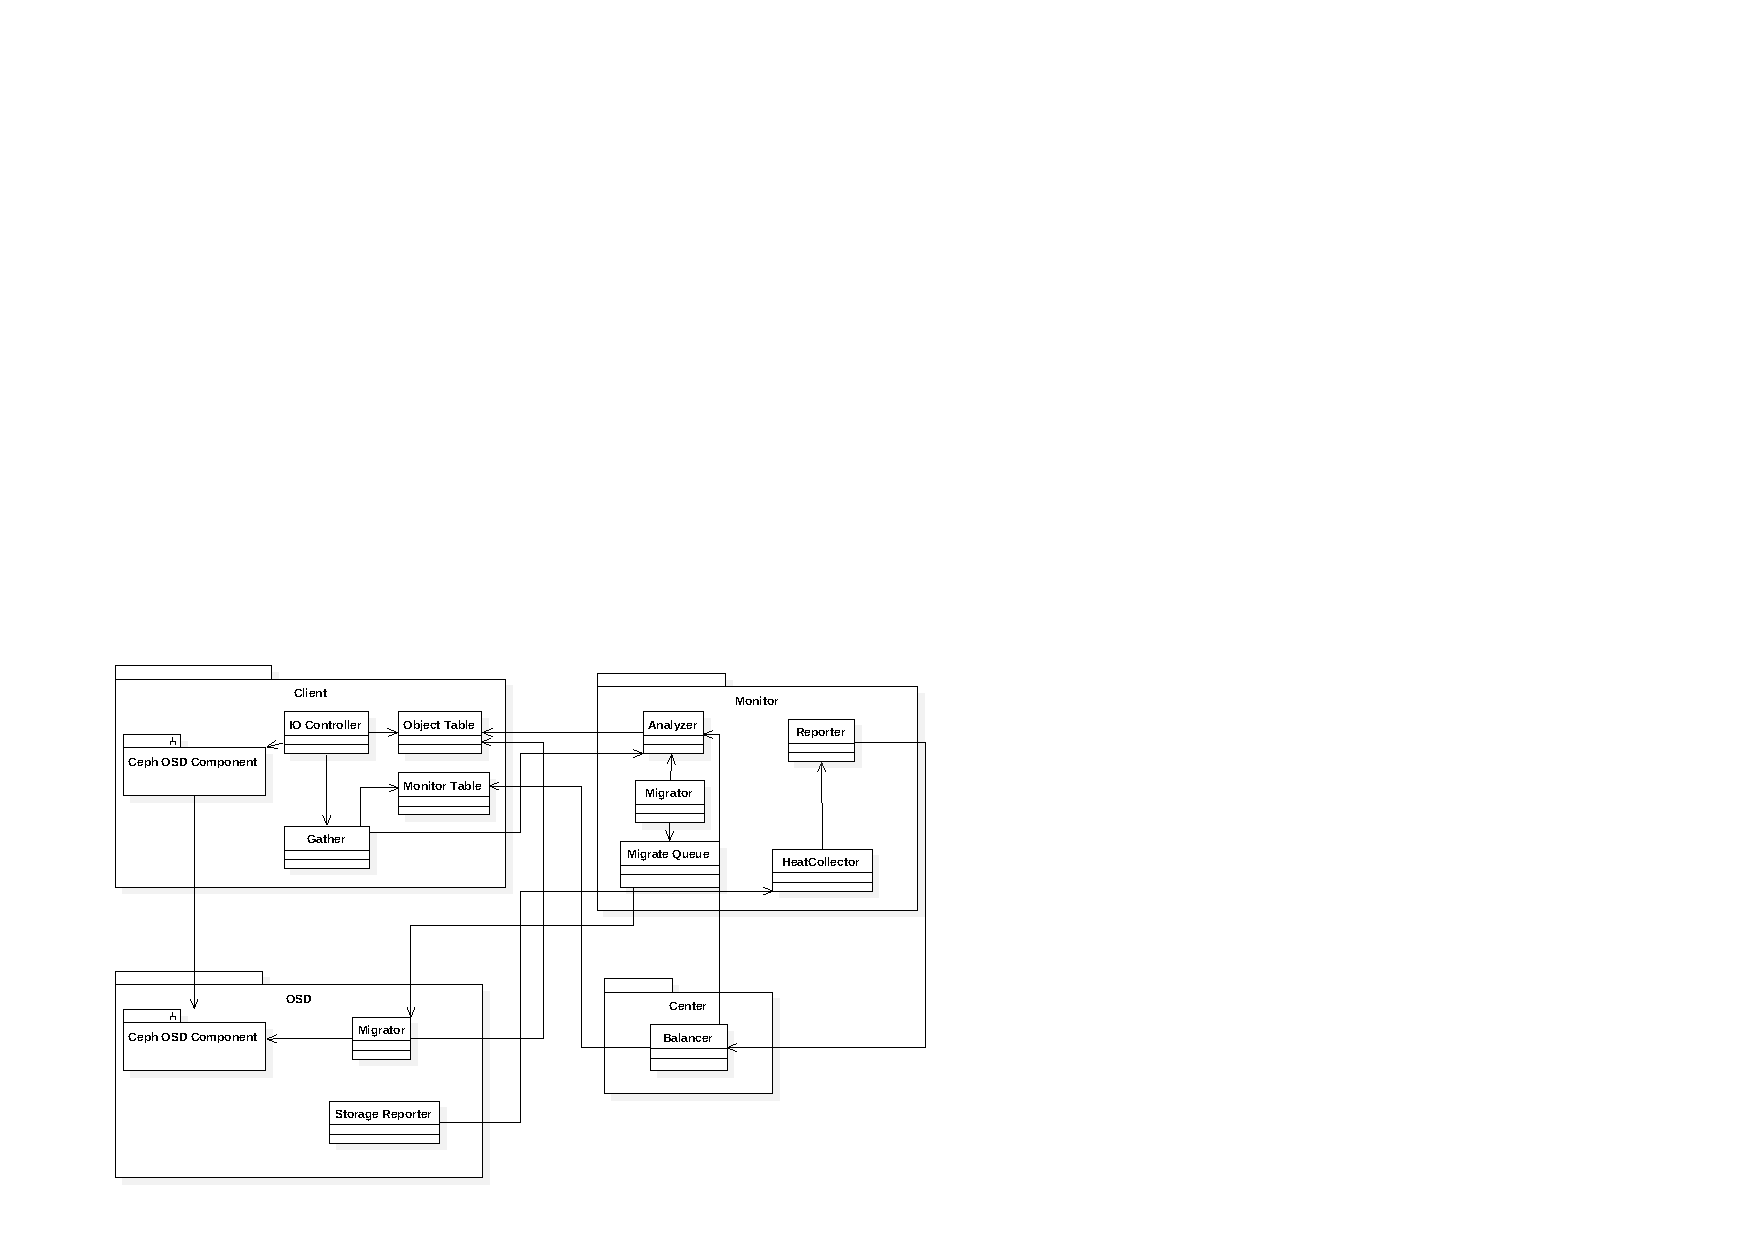
\includegraphics[width=15cm]{example/implmain.pdf}
    \bicaption[fig:implmain]{DOBBS模块结构}{DOBBS模块结构}{Fig}{Module Structure of DOBBS}
\end{figure}

Client主要包含四个类,这四个类也是与系统设计中的模块一一对应的。IO Controller用来截取VM的数据请求,并通过查询Object Table的方式来获取对象所在的OSD编号,再把对象ID和所在OSD编号共同
传递给Ceph OSD Component进行数据访问。IO Controller还有就是需要调用Gather的接口来记录VM访问对象的访问类型和ID,因此IO Controller没有暴露给外部的接口,它则主要对Ceph和QEMU源代码的修改。
Object Table的主要作用是保存一个对象ID到OSD ID映射的数据结构,并暴露出可以让IO Controller进行查询的接口,另外在局部热均衡对象迁移结束之后OSD上的Migrator也需要调用Object Table提供的更新映射的接口。
Gather则用于收集对象的访问信息,并调用Monitor上的接口将单位时间的数据流信息汇报给Monitor的Analyzer。而Monitor Table是用于存储Monitor ID与OSD ID的数据结构,因为全局热均衡会改变系统的逻辑结构,所以在全局热均衡结束之后会去更新Monitor Table提供的更新映射的接口。Gather则用于收集对象的访问信息,并调用Monitor上的接口将数据汇报给Monitor
,Gather在汇报给Monitor的之前需要先通过对象的OSD查询Monitor Table得到到该OSD在哪个子集群,然后在将相同子集群的对象数据流信息整合起来打包发送给对象的Monitor。

Monitor则包含五个类。Analyzer是用于接收Client的Gather所汇报的数据流信息,并且它内部会持续计算对象热度,在生成对象迁移策略之后调用Migrator发送迁移请求,Analyzer的另一个重要功能就是接受Center节点的命令开始热扩散的使能过程。
Migrator则主要负责对象的迁移请求发送等。Migrator Queue的主体是一个队列,用于存储迁移请求,另外Migrator Queue还会额外记录子集群当前迁移数量。Heat Collector是在全局热均衡中所用的类,它的主要作用是调用操作系统
指令获得Monitor的CPU和内存利用率,还有就是调用所在子集群OSD上的Storage Reporter接口获取存储设备的IOPS。Reorter则是会调取HeatCollector提供的接口获得实时子集群热度值,并定时将这个值
发送给Center的Balance。Center上的Balancer的主要功能就是接受Monitor发送的子集群热度值,然后运行算法\ref{algo:imbadect}生成热扩散请求,在热扩散结束之后再修改所有Client上的Monitor Table。


\subsection{Monitor的模块实现}
\begin{figure}[!htp]
    \centering
    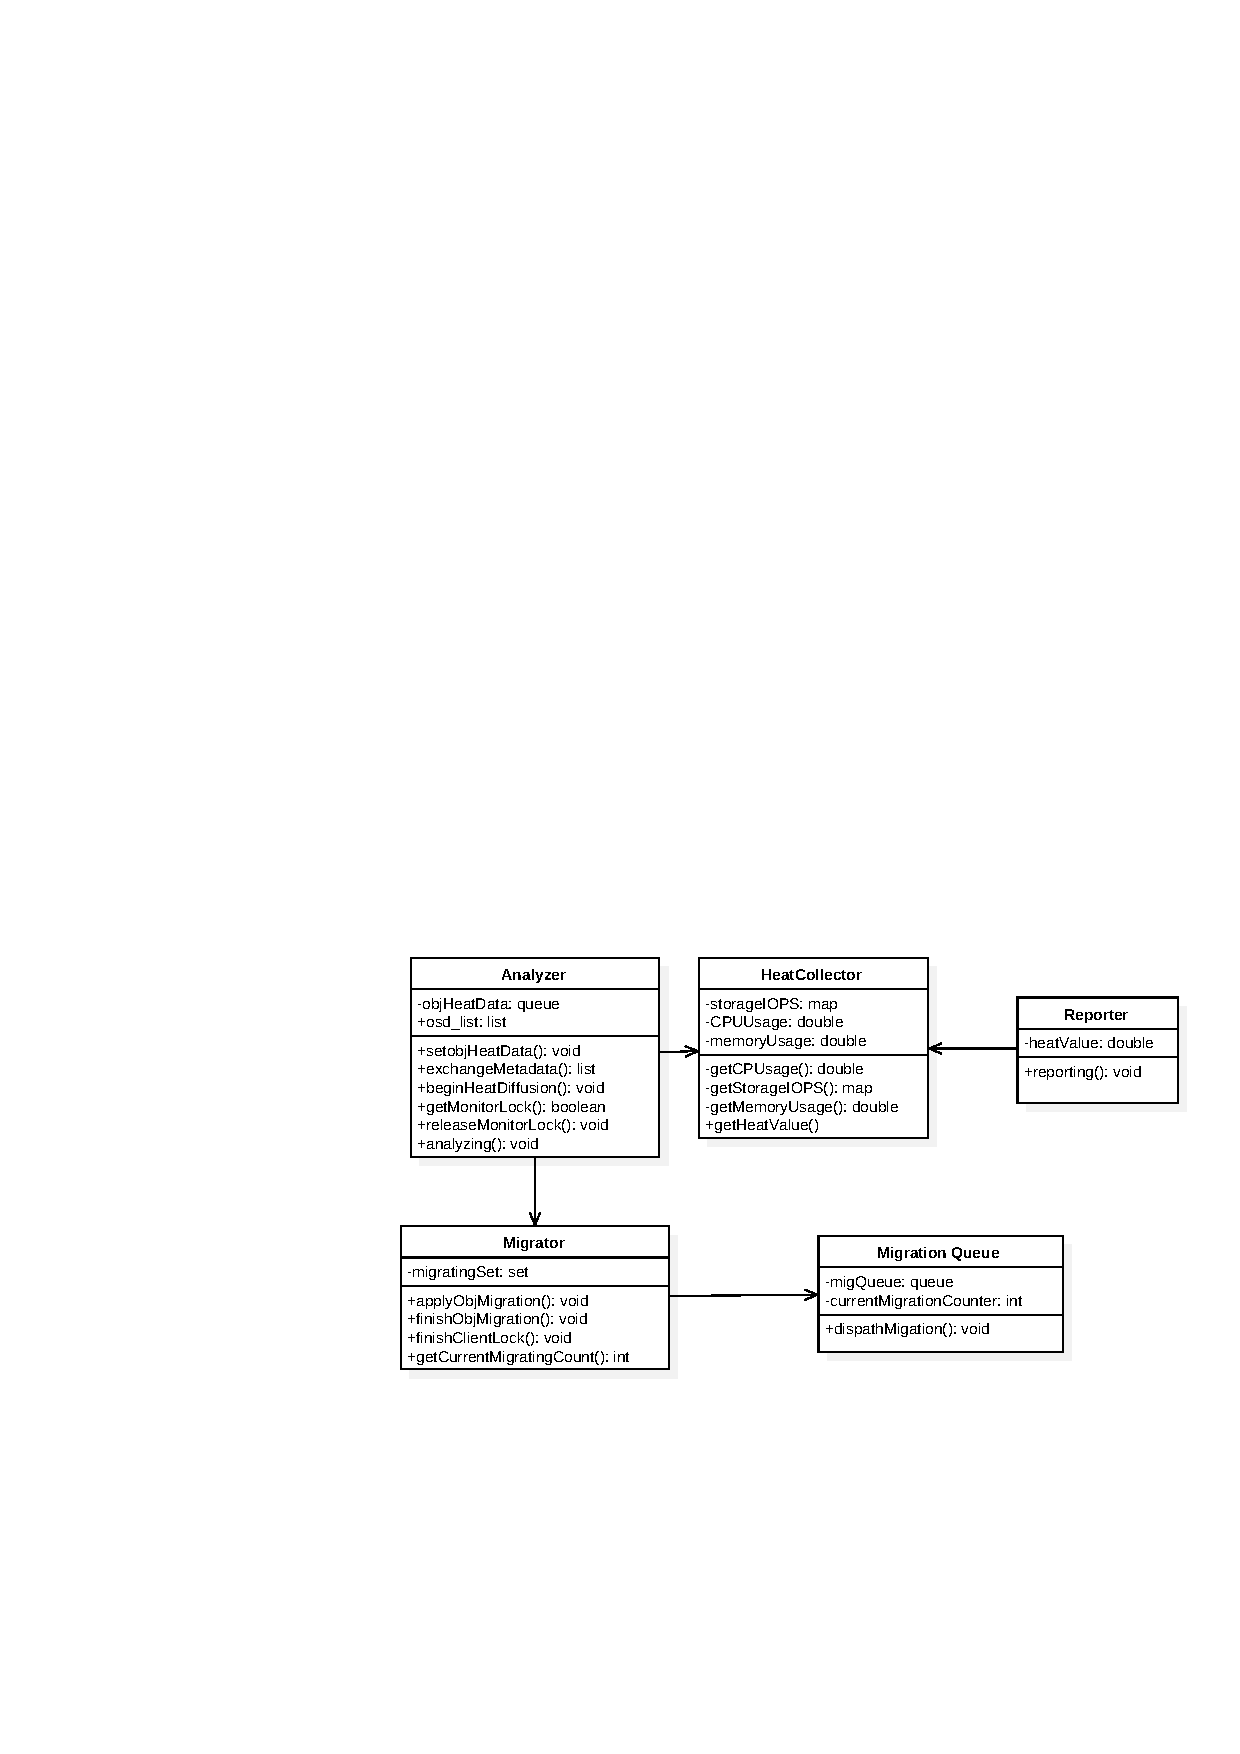
\includegraphics[width=14cm]{example/implmon.pdf}
    \bicaption[fig:implmon]{监视器模块类图}{监视器模块类图}{Fig}{Class Diagram of Monitor}
\end{figure}

图\ref{fig:implmon}所示是Monitor模块的设计类图。从图中可以看到Monitor一共有五个主要的类,其中的Analyzer、Migrator和Migrator Queue是继承于WHOBBS的实现\cite{lingxuan2015whobbs}。在本小结中,我们只做
简单的介绍,但是我们扩展了原有Analyzer类的功能,如全局热均衡的使能过程。

\subsubsection{Analyzer}
Analyzer的主要功能就是在局部热均衡的时候保存数据对象的热度信息,然后不断分析所有数据对象,计算对象的热度,并产生对象迁移请求。objHeatData是一个有序队列,我们实现了一个叫做ObjectQueue<typename T>的内置类,它内部是通过链表实现的
队列结构,只不过在链表插入的时候是根据元素的热度值进行的降序排序,保证了对头的元素的热度值总是最大的。objHeatData实际上的类型是ObjectQueue<ObjInfo>,ObjInfo是我们用来表示对象热度信息的结构体,这个结构体包含对象ID(oid)、所在
OSD编号(osd\_id)、所属Client IP(client\_ip)和热度(heat\_val)。因此objHeatData是用于存储对象热度信息的,它通过heat\_val降序排序。Analyzer还有个数据结构是osd\_list,它的类型是std::list<int>,它用来存储当前子集群所包含的OSD
编号。

analyzing()方法是一个线程入口函数,Analyzer在被实例化之后就会启动分析线程。分析线程工作就是不断遍历objHeatData,产生对象迁移请求。根据上一章对Monitor的设计,analyzing遍历时候的策略就是将会维护一个当前SSD剩余容量的计数,在SSD的容量
没有满的时候,它会把objHeatData的前若干个对象放置于SSD上。然后在该线程内部也会有两个集合,分别表示当前在SSD中的对象和在HDD中的对象。通过前面的策略,很快SSD就会被填满。
一旦SSD的容量已满,该线程则会遍历objHeatData的前N个对象,N的大小等于SSD容量/单个对象大小,找到这前N个对象中哪些是在SDD上哪些是在HDD上。如果出现HDD上的对象位于前N的位置,则将该对象从HDD迁移到SSD上。如果发现SSD集合中的对象不在前N的位置里,
则将该对象迁出SSD\cite{lingxuan2015whobbs}。该分析线程发送迁移指令是通过调用Migrator的applyObjMiration()的接口来实现的。setObjData()接口的实现相对简单,它只是用来在Monitor接收到Client汇报来的数据流对象,通过热度计算算法计算出每个对象的热度之后,如果objHeatData中含有这个对象
则更新它的热度值,否则实例化一个ObjInfo对象,将它插入到objHeaData中。值得注意的是,objHeatData的插入过程我们用到的是插入排序算法,从而保证每次插入都是有序的。

beginHeatDiffusion()、getMonitorLock()、releaseMonitorLock()和exchangeMetadata()这四个接口是Center所调用的。getMonitorLock()是用于对局部热均衡上锁,它会先去调用Migrator的getCurrentMigratingCount()接口获取现在子集群是否还有正在迁移的对象,如果接口返回值非0,则
不能上锁,接口返回false。如果getCurrentMigratingCount()的返回值是0,则会对analyzing()上锁并返回true,上锁我们是通过Linux的互斥锁pthread\_mutex\_t来实现的。beginHeatDiffion()接口是Center检测到子集群热度不均衡之后,并对Monitor
上锁之后执行的接口。这个接口就是全局热均衡使能过程的开始。而releaseMonitorLock()接口是Center在全局热均衡使能过程之后用于释放Monitor锁的,它调用pthread\_mutex\_unlock()这个Linux线程函数来解除加载analyzing线程上的互斥锁。这个互斥锁
是用在Analyzer的objHeatData这个数据结构上的,在上锁之后其他线程就不能对objHeatData进行读写操作,从而局部热均衡将被暂停。

beginHeatDiffusion()接口传入的参数是目标子集群Monitor的IP地址。在接口开始调用的时候,它会调用HeatCollector的getStorageIOPS()接口,这个接口会返回子集群的存储集群各个OSD的编号和IOPS的映射。在获得这个映射之后,它找到最大IOPS的OSD编号。
然后它会去objHeatData中去遍历,找到所有osd\_id为IOPS最大OSD的对象,将它们从队列中剔除并置于一个传输buffer中。这个buffer实际上类型为std::list<ObjInfo>的对象。封装完成后,它通过Thrift调用目标子集群Monitor的exchangeMetadata()接口以参数的方式将buffer中的元数据传输给目标子集群。目标子集群
会从接口exchangeMetadata()返回其最“冷”OSD所对应的元数据,返回值类型为std::list<ObjInfo>,然后将源子集群发送来的元数据调用setobjHeatData()接口插入objHeatData中。
beginHeatDiffusion()在接受到目标子集群的返回值之后,它把列表中的数据插入其自身的objHeatData,在接口执行的最后它会更新osd\_list中值,最后它调用Center的finishDiffusion()
方法,通知Center热扩散的使能过程已经完成。exchangeMatadata()接口则是在目标子集群的Monitor上被调用的接口,它的参数是源子集群最“热”OSD对应的元数据。该接口被调用之后,它会通过查询HeatCollector,找到IOPS最低的OSD编号,并将它所对应的元数据从onjHeatData中剔除,并通过返回值的方式传送给源子集群。

\subsubsection{Migrator和Migrator Queue}
Migrator和Migrator Queue的实现与WHOBBS中的实现相似,我们这里不再详细叙述这两个模块的实现。Migrator主要向Analyzer提供applyObjMigration()接口,Analyzer调用该接口后,该接口的传入参数是一个表示对象迁移的数据结构,它包括被迁移对象的原OSD编号、目的OSD编号和对象ID,
,然后它会调用Client上的对象上锁接口,在上锁成功后将迁移请求(表示迁移的数据结构)放置于Migrate Queue。
finishObjMigrating()接口是在OSD结束对象传输之后调用的,调用之后会把这个对象从migratingSet中剔除,然后调用Client上的释放锁的接口\cite{lingxuan2015whobbs}。与WHOBBS不同的是,为了支持Monitor锁,我们增加了getCurrentMigratingCount()接口,这接口在调用之后会直接返回当前migratingSet的大小。
migratingSet是在发送请求之后将oid放入其中,直到迁移完成后才会把它从migratingSet删除掉,因此migratingSet表示的是当前正在迁移对象的ID。Migrator Queue的实现与WHOBBS无异,本文则不再叙述。

\subsubsection{HeatCollector}
HeatCollector的功能是获取子集群的所有事实资源信息的。它主要有三个成员变量,分别是storageIOPS(存储集群IOPS)、CPUUsage(Monitor的CPU利用率)和memoryUsage(Monitor的内存利用率)。其中storageIOPS的数据类型是std::map<int, long>,这个map数据结构的键为osd\_id,值为对应OSD的IOPS值。
CPUUsage和memoryUsage的类型都是double,即占用百分比。

getHeatValue()是HeatCollector对外提供的接口,该接口被调用之后,它会依次调用getStorageIOPS()、getCPUUsage()和getMemoryUsage()接口获得当前实时的子集群资源信息,并更新它的三个成员变量。对于getStorageIOPS(),它会从在Analyzer的osd\_list获取子集群所包含OSD的编号,
然后再调用本子集群的OSD上的getIOPS()接口,最后将最新的存储集群IOPS值以map的方式返回。getCPUUsage()接口则是调用Linux的系统调用查看/proc/stat文件来获取当前CPU利用率。getMemoryUsage()则调用sysinfo()系统调用来获得当前的内存利用率的。在getHeatValue()成功调用这些接口
之后,它会根据公式\ref{eq:stheat}计算当前实时的热度值并返回给调用者。

\subsubsection{Reporter}
Reporter的功能则是汇总子集群的资源利用信息,并定时发送给Center。Reporter包含一个成员变量,就是当前子集群的实时热度是heatValue,它的类型是double。reporting()函数是一个线程入口函数,该线程的主要功能就是不断的调用HeatCollector的getHeatValue()接口,在每次获取之后都会调用Center的reportFromMonitor()接口把热度值传输给Center。

\subsection{Center模块实现}

\begin{figure}[!htp]
    \centering
    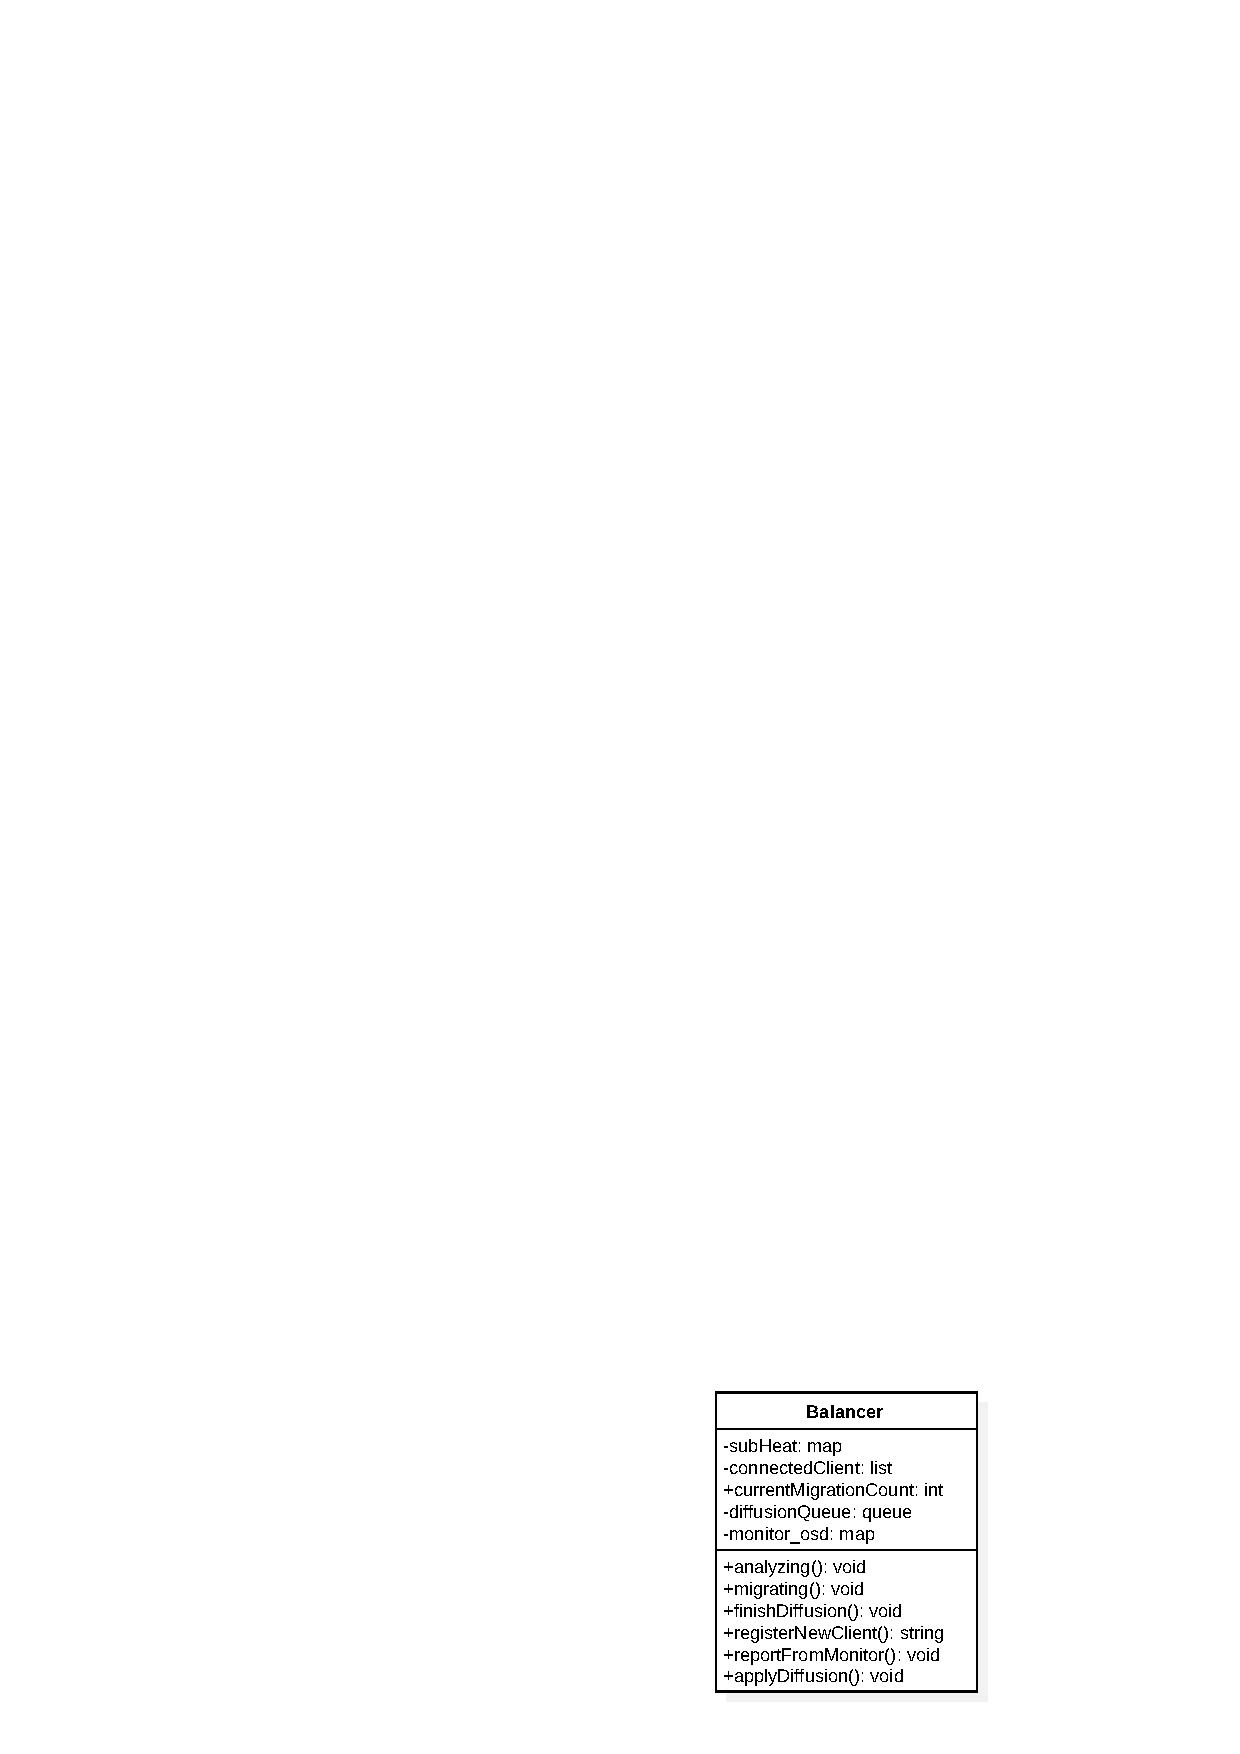
\includegraphics[width=5cm]{example/implcenter.pdf}
    \bicaption[fig:implcenter]{中心模块类图}{中心模块类图}{Fig}{Class Diagram of Center}
\end{figure}

如图\ref{fig:implcenter}所示为DOBBS的Center模块的类图,从图中可以看到Center只有一个叫做Balancer的类。Balancer类就实现了Center的所有功能,包括对各个子集群热度信息的收集、产生热迁移请求和新Client接入时的分配。

\subsubsection{Balancer}
Balancer主要有subHeat、connectedClient、currentDiffusionCount、diffusionQueue和monitor\_osd等五个成员变量。subHeat的数据类型的std::<std::string, double>,它表示各个子集群的热度值,其中的键为子集群id,值为热度值。connectedClient,它的类型是
std::list<std::string>表示当前接入系统的Client的IP地址。currentDiffusionCount表示当前正在全局热均衡的请求数量,它的类型是int。diffusionQueue表示准备进行热扩散的队列,它的类型是std::queue<DiffusionDetail>,DiffusionDetail是一个用来表示热扩散请求的结构体,
它包含to\_sub和from\_sub,即源子集群和目标子集群的编号。

Balancer的analyzing()函数是一个线程入口函数,这个线程主要就是用来运行子集群热度不均衡检测算法\ref{algo:imbadect},当算法找到源子集群和目的子集群之后会把原子群和目标子集群标号通过参数的方式传递给接口applyDiffusion()。而analyzing线程会过一定时间间隔
执行一次热度不均衡检测算法。reportFromMonitor()接口则是用于持续接受,各个Monitor所汇报的热度值信息。

applyDiffusion()算法在接收到源子集群编号和目标子集群编号之后,会生成一个DiffusionDetail类型的结构体,该结构体包含to\_sub(目标子集群)、from\_sub(源子集群)这两个信息,并将其放置于diffusionQueue中。migrating()函数则是迁移线程的入口函数,它的工作就是不断轮训diffusionQueue的内容,只要队列不为空它
会先检查currentDiffusionCount的值是否达到系统最大热扩散数量,如果已经达到则不对队列做任何处理。如果currentDiffusionCount小于系统最大热扩散数量,那么它会通过子集群编号调用两个子集群的getMonitorLock()接口,只有当两个都返回true时才将
这个热扩散请求从diffusionQueue删除。在这之后,它会调用源子集群的beginHeatDiffsion()接口,并将目标子集群标号传递给它。

finishDiffusion()接口是在源子集群和目标子集群结束全局热均衡的使能过程之后调用的,最终是由源子集群调用。在调用之后,Center会首先更新monitor\_osd的值,因为全局热均衡已经修改了子集群的逻辑结构。然后,Center再去更新通过connectedClient列表
去更新所有连接的Client的MonitorTable。最后则是调用目标子集群和源子集群的releaseMonitorLock()接口对两个Monitor解锁。

在上一章已经讲过,当Client初次接入系统时,Center会分配一个相对较“冷”的子集群给这个Client。在Client初次接入时,它会调用registerNewClient()接口,再把自己的IP地址通过传参的方式发送给Center。这个接口会遍历subHet,找到一个热度值最低的
子集群,然后将这个子集群Monitor的id返回给Client,最后Center把这个Client的IP置于connectedClient中。

\subsection{Client模块实现}
\begin{figure}[!htp]
    \centering
    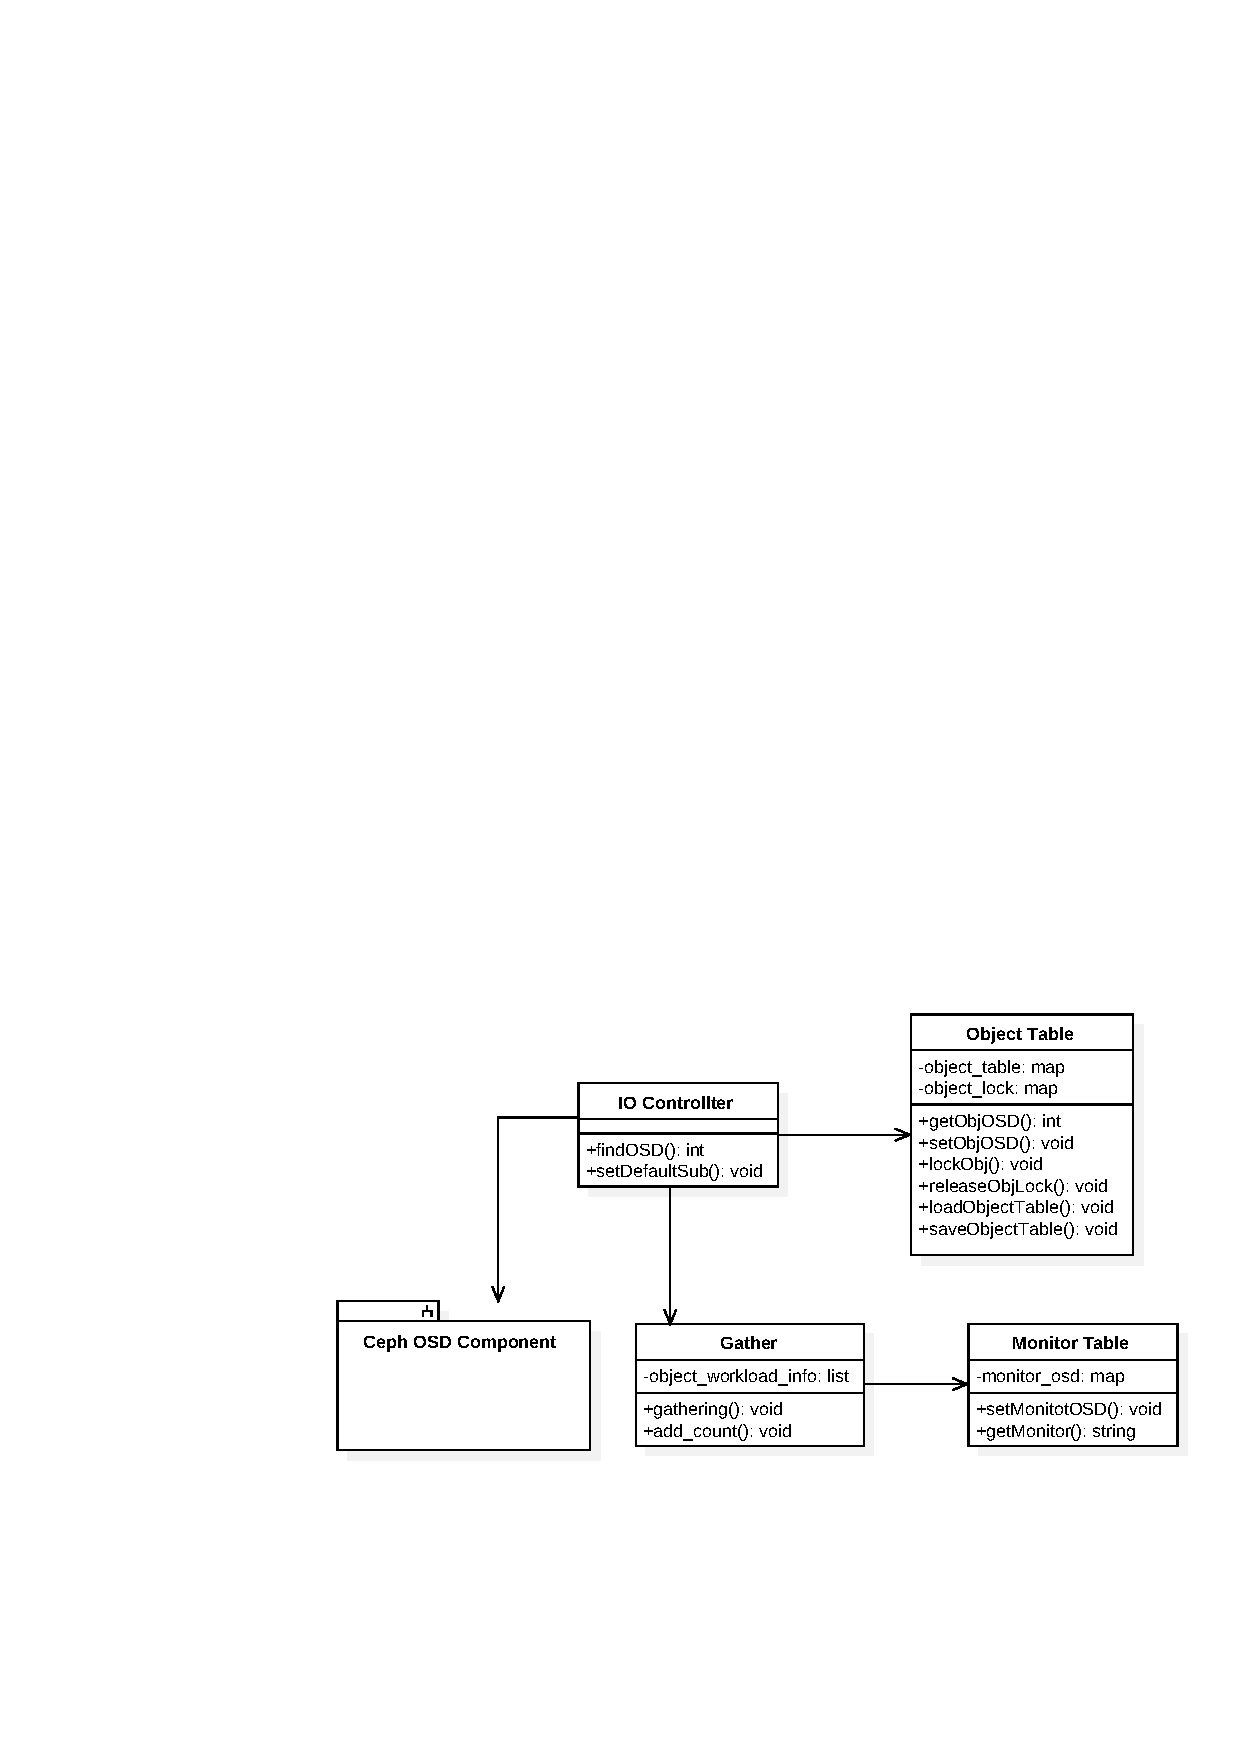
\includegraphics[width=12cm]{example/implclient.pdf}
    \bicaption[fig:implclient]{客户端模块类图}{客户端模块类图}{Fig}{Class Diagram of Client}
\end{figure}

如图\ref{fig:implclient}为Client模块的类图。Client模块是运行虚拟机和虚拟机管理器的模块,该模块的IO Controller、Object Table和Gather这三个类的实现与WHOBBS基本一致,所以本文不再过多赘述。但是,我们在原有实现的基础上加入了Monitor Table类,用于负责全局热均衡后系统的OSD和Monitor之间
的变化。

因为Client的设计,我们要截取VM对对象访问的请求,这就需要我们对Ceph的原生代码做出修改。我们主要修改了Ceph librbd模块的代码,在Ceph调用底层对象传输之前,我们让它先调用IO Controller的findOSD()接口。IO Controller的findOSD()接口是以对象ID
作为参数,然后在Object Table中调用getObjOSD()接口进行查询对象当前所对应的OSD编号,然后返回给Ceph之后,再进行后续的对象访问。值得注意的是,因为DOBBS的多Monitor设计,以及静态全局热均衡,所以我们需要在Client初次接入系统的时候可以获得它所在的默认
子集群。因此,与WHOBBS不同,我们在IO Controller加入了一个接口setDefaultSub()这个是用于Center设置当前Client默认子集群的接口。当然,为了在Client第一次接入DOBBS才会去向Center获得默认子集群编号,我们也对Ceph的源代码进行了修改。

Object Table的实现与WHOBBS没有区别,本文仅介绍各个接口的作用,具体细节不再介绍。首先,该类包含两个成员变量,分别是object\_table和object\_lock。它们都是std::map的数据结构,object\_table是用来保存对象ID和OSD编号的映射关系,而object\_lock并
不保存信息,只是保存哪些对象上了锁。而getObjOSD()和setObjOSD()则是对object\_table进行操作,分别是通过对象ID获取对应的OSD编号,还有就是修改object\_table的内容。lockObj()和releaseObj()这两个接口都是在局部热均衡过程中保证一致性对对象上锁和解锁
所用到的接口。loadObjTable()和saveObjTable()则是用于在DOBBS系统启动和关闭后将object\_table存盘和读取的接口。

我们在WHOBBS原有Gather类的基础上进行了扩展。gather()是线程入口函数,它的功能就是定时向Monitor发送对象的数据流信息。我们定义对象的数据流信息包括,对象ID(oid)、OSD ID(sid)、访问类型(access\_type)、访问次数(access\_count)。与WHOBBS不同,在WHOBBS中只有一个
Monitor存在,所以所有Client都只需要向同一个Monitor发送自己的数据流信息。对于DOBBS,我们的Monitor会有多个,而且由于全局热均衡,OSD也会随之发生变化。在DOBBS的设计中,OSD是与子集群绑定的,所以我们需要保证Client可以实时知道每个OSD都在哪个子集群中。
Monitor Table就是用来保存子集群和OSD的信息。gather线程在每次向Monitor发送之前,都会通过Monitor Table查询到当前对象所在的OSD位于哪个子集群,然后将相同子集群的对象数据流信息组合成一个列表共同发送给对应的Monitor。

Monitor Table类的主要功能,首先是保存当前最新的OSD和子集群的信息,其次就是接受来自Center的更新,还有就是Gather会来查询。它有一个叫做monitor\_osd的成员变量,它的类型是std::map<std::string, std::string>,它存储了OSD ID到子集群Mointor的IP地址之间的映射关系。
setMonitorOSD()接口是由Center远程调用的,在全局热均衡的使能过程之后Center会通知所有连接到系统的Client更新各自的Monitor Table。getMonitor()接口则是开放给Gather用于查询对象所在子集群的,它传入的参数是OSD ID,返回值为Monitor的IP地址。

\subsection{OSD模块实现}
对于OSD模块的实现,我们完全沿用了WHOBBS的实现方案没有做更多的扩展,所以本小节只做简要的概括。可以从图\ref{fig:implmain}中看到,OSD上的Migrator负责接收来自于Monitor的迁移请求,在接收到之后,它只需要调用Ceph的OSD组件即可完成对象的迁移。而Storage Reporter则是调用了
操作系统指令获得当前磁盘(SSD/HDD)的IOPS值。Monitor上的Heat Collector类会远程调用Storage Reporter的接口获得当前的IOPS值。

\section{系统主要工作流程}
本小结主要介绍DOBBS的主要工作流程。局部热均衡中的工作流程,如对象的迁移、对象数据流信息的获取以及虚拟机的IO请求这些工作流程与WHOBBS中的实现并没有太大的区别,所以本小节对局部热均衡的工作流程只是做一个高度的概括,而不做过多的描述。
全局热均衡是一个复杂的过程,我们将它抽出三个比较主要的工作流程来进行介绍,分别是客户端接入工作流程、监控器获得并汇报子集群热度信息工作流程和全局热均衡使能过程工作流程。客户端接入过程,是静态的全局热均衡的保证并且还是让
客户端可以顺利与系统交互的重要保证。监控器获得并汇报子集群热度信息的过程也就是Center获得各个子集群热度的过程,这对Center进行子集群热度不均衡检测尤为重要。全局热均衡使能过程是全局热均衡最重要的一环,本小结从Center发出
迁移指令开始来叙述全局热均衡的使能过程。

\subsection{局部热均衡工作流程}

局部热均衡的工作流流程主要可以分为以下几个部分:虚拟机IO请求工作流、虚拟机汇报对象数据流信息工作流以及对象迁移工作流。虚拟机IO请求工作流一般是由虚拟机发起的,然后IO Controller先去查询Object Table,找到该对象对应的
OSD ID,然后将OSD ID返回给IO Controller,最后IO Controller将对象ID和OSD ID以参数的方式调用Ceph OSD Component接口,来进行后续的访问。在这个过程中,IO Controller起到的是截取请求的作用。值得注意的是,因为我们要
获得对象的访问信息,所有在IO Controller的findDefaultOSD()被调用的时候,它还会调用Gather的add\_count()接口,把当前虚拟机所访问的对象ID和访问类型传递给Gather。


虚拟机汇报对象数据流信息工作流则相对简单,Gather的gathering线程会定时将储存的对象数据流信息发送给Monitor的Analyzer,而每次发送之后它都会清空之前的记录。对象迁移工作流则是局部热均衡的重点。Analyzer在得出迁移策略之后,它会
调用Migrator,Migrator生成迁移请求,然后Migrate Queue把迁移请求缓存下来,如果子集群当前的迁移数量小于最大迁移数量则开始迁移。首先,调用Client上的lockObj()接口,之后向该对象对应的OSD发送请求,OSD调用Ceph OSD Component进行
对象迁移,迁移结束后OSD调用Migrator的finishObjMigration()接口,最后再对Client上的对象解锁。

\subsection{客户端接入工作流程}
\begin{figure}[!htp]
    \centering
    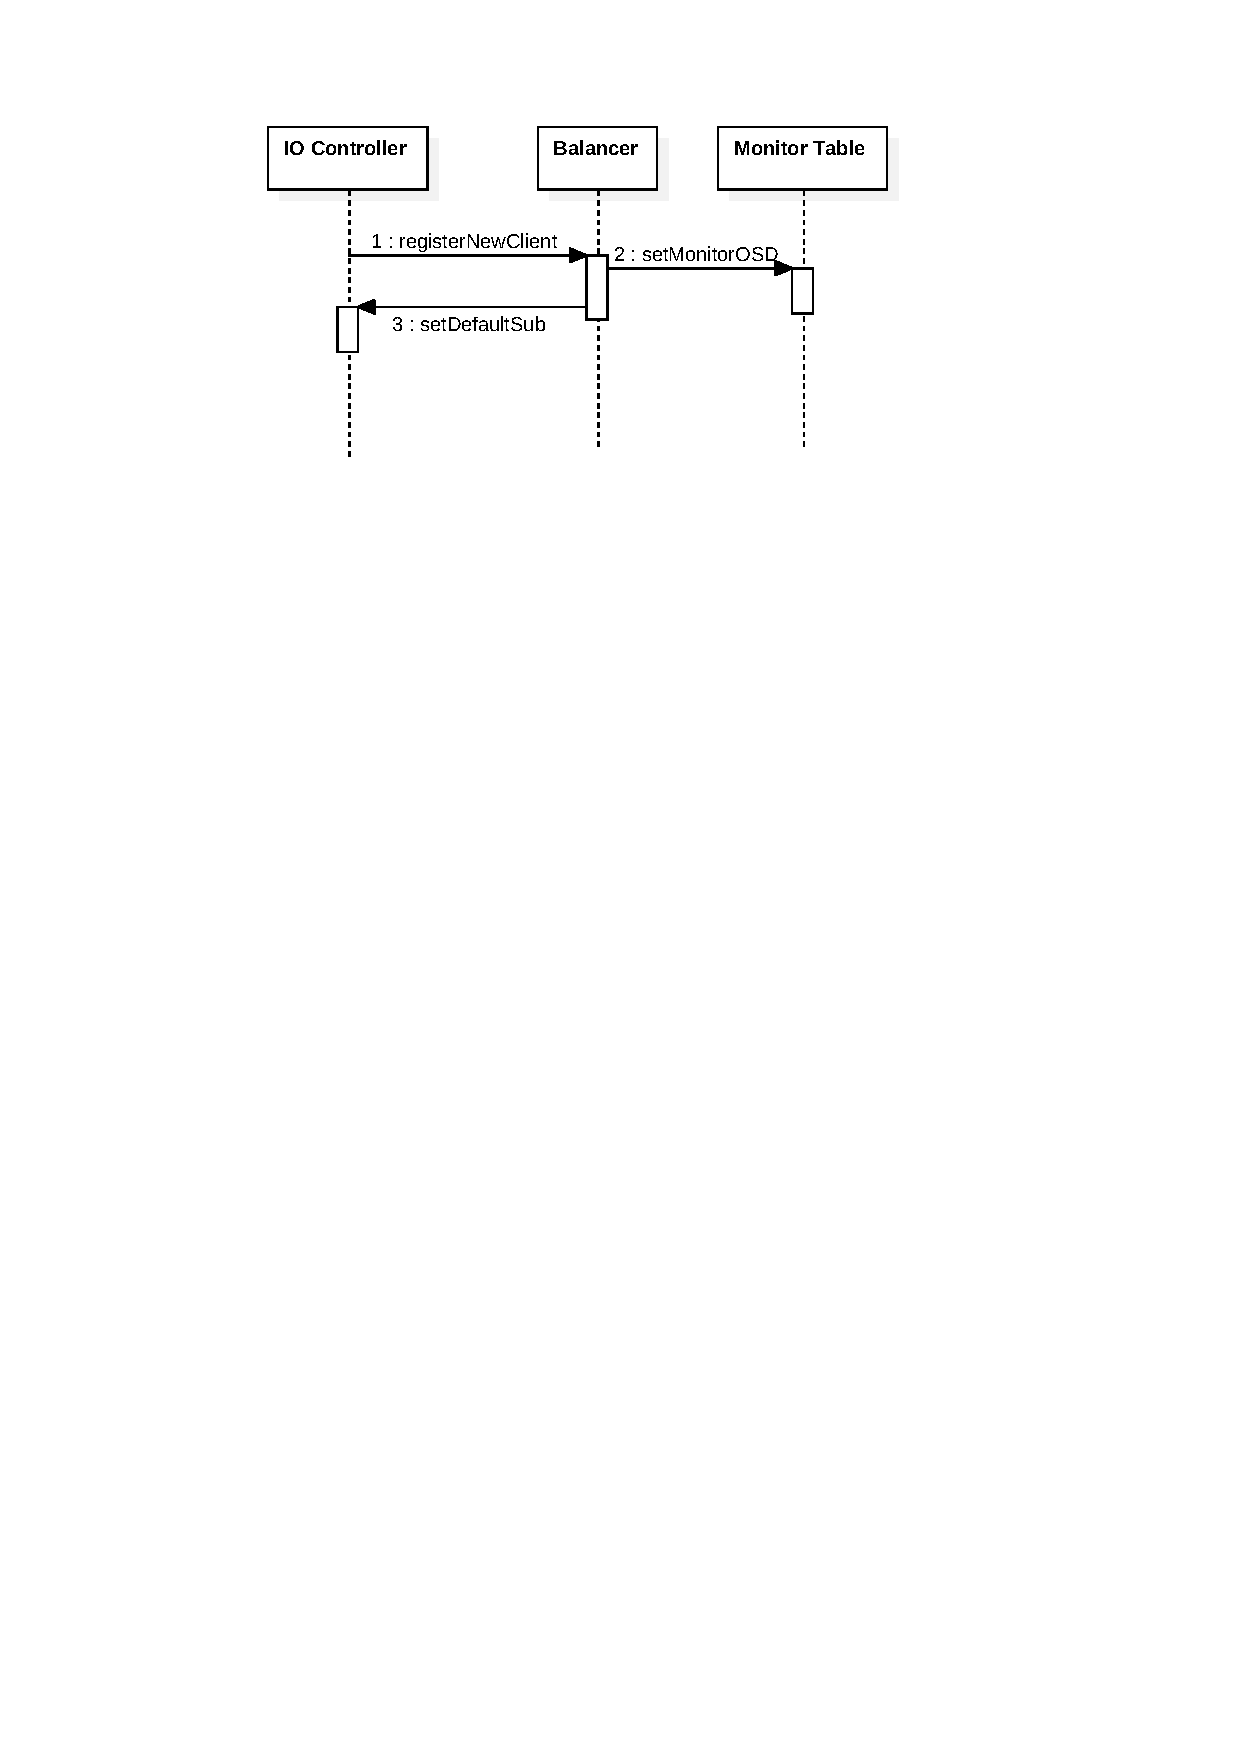
\includegraphics[width=10cm]{example/seqinit.pdf}
    \bicaption[fig:seqinit]{客户端接入的工作流程}{客户端接入的工作流程}{Fig}{The Work Flow of Client First Access}
\end{figure}

客户端初次接入DOBBS的工作流程如图\ref{fig:seqinit}所示。从图中可以看到,IO Controller会首先调用Center的Balancer的registerNewClient()接口,然后该接口通过查询subHeat,将当前热度值最低的子集群发送给IO Controller。同时,
它会把请求接入的Client的IP地址写入connetedClient中,然后把当前系统最新的monitor\_osd通过调用setMonitorSub()发送给这个初次接入的Client。

\subsection{监控器获得并汇报子集群热度信息工作流程}

图\ref{fig:seqhet}所示,是子集群的Monitor向Center发送当前子集群热度值的工作流程,这个工作流程还包括Monitor的HeatCollector定期从子集群的OSD中获取IOPS信息,并根据
公式\ref{eq:stheat}计算子集群热度,最后再把计算好的热度值通过Thrift提供的远程调用接口发送给Center。

对于该工作流,值得注意的是Reporter发起的getUsage请求是由Reporter的reporting线程发送的,reporting线程则是以固定的时间间隔发起getUsage请求。HeatCollector在收到请求
之后,会先去在Analyzer上去查询本子集群有哪些OSD。在这之后,它会通过查询到的OSD列表调用每个OSD上的getStorageIOPS()接口,接口返回后,HeatCollector将其记录并依次调用getCPUUsage()
和getMemoryUsage()接口,最后通过公式计算出热度值并调用Center的reportFromMonitor()接口将它传输给Center。

\begin{figure}[!htp]
    \centering
    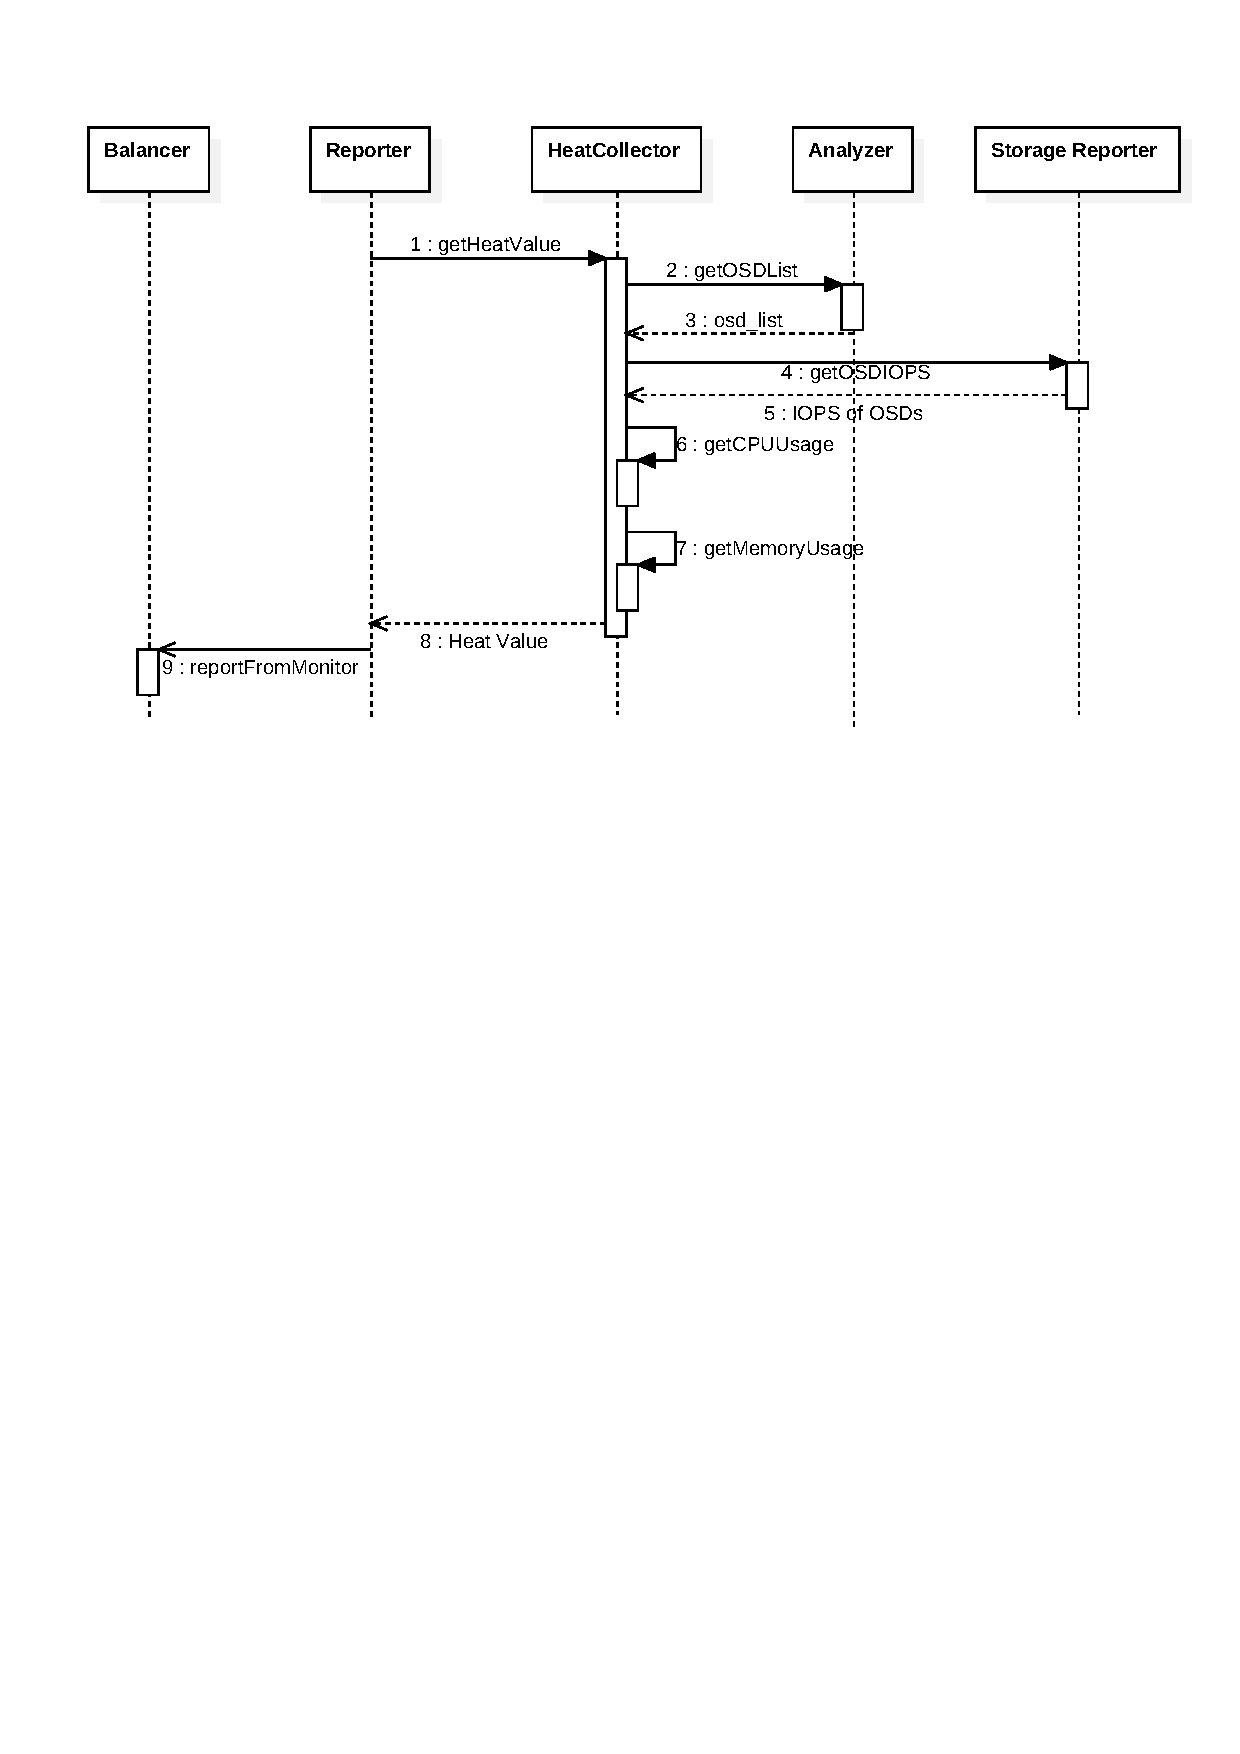
\includegraphics[width=12cm]{example/seqhet.pdf}
    \bicaption[fig:seqhet]{监控器获得并汇报子集群热度信息工作流程}{监控器获得并汇报子集群热度信息工作流程}{Fig}{The Work Flow of Monitor Reports Heat}
\end{figure}

\subsection{全局热均衡使能过程工作流程}


全局热均衡是本论文的一个核心概念,而全局热均衡的使能过程更是关键。图\ref{fig:seqghb}所示为全局热均衡的使能过程的工作流程。在Balancer的不均衡检测算法检测出不均衡之后,就
启动了使能过程。首先就是为了解决迁移过程中的一致性问题,我们用try-lock机制来对Monitor上锁。但是图\ref{fig:seqghb}中,我们假设的是成功上锁之后的工作流程。如果不能成功地从
目标子集群和源子集群获得锁,则不会进行后续的使能过程。
\begin{figure}[!htp]
    \centering
    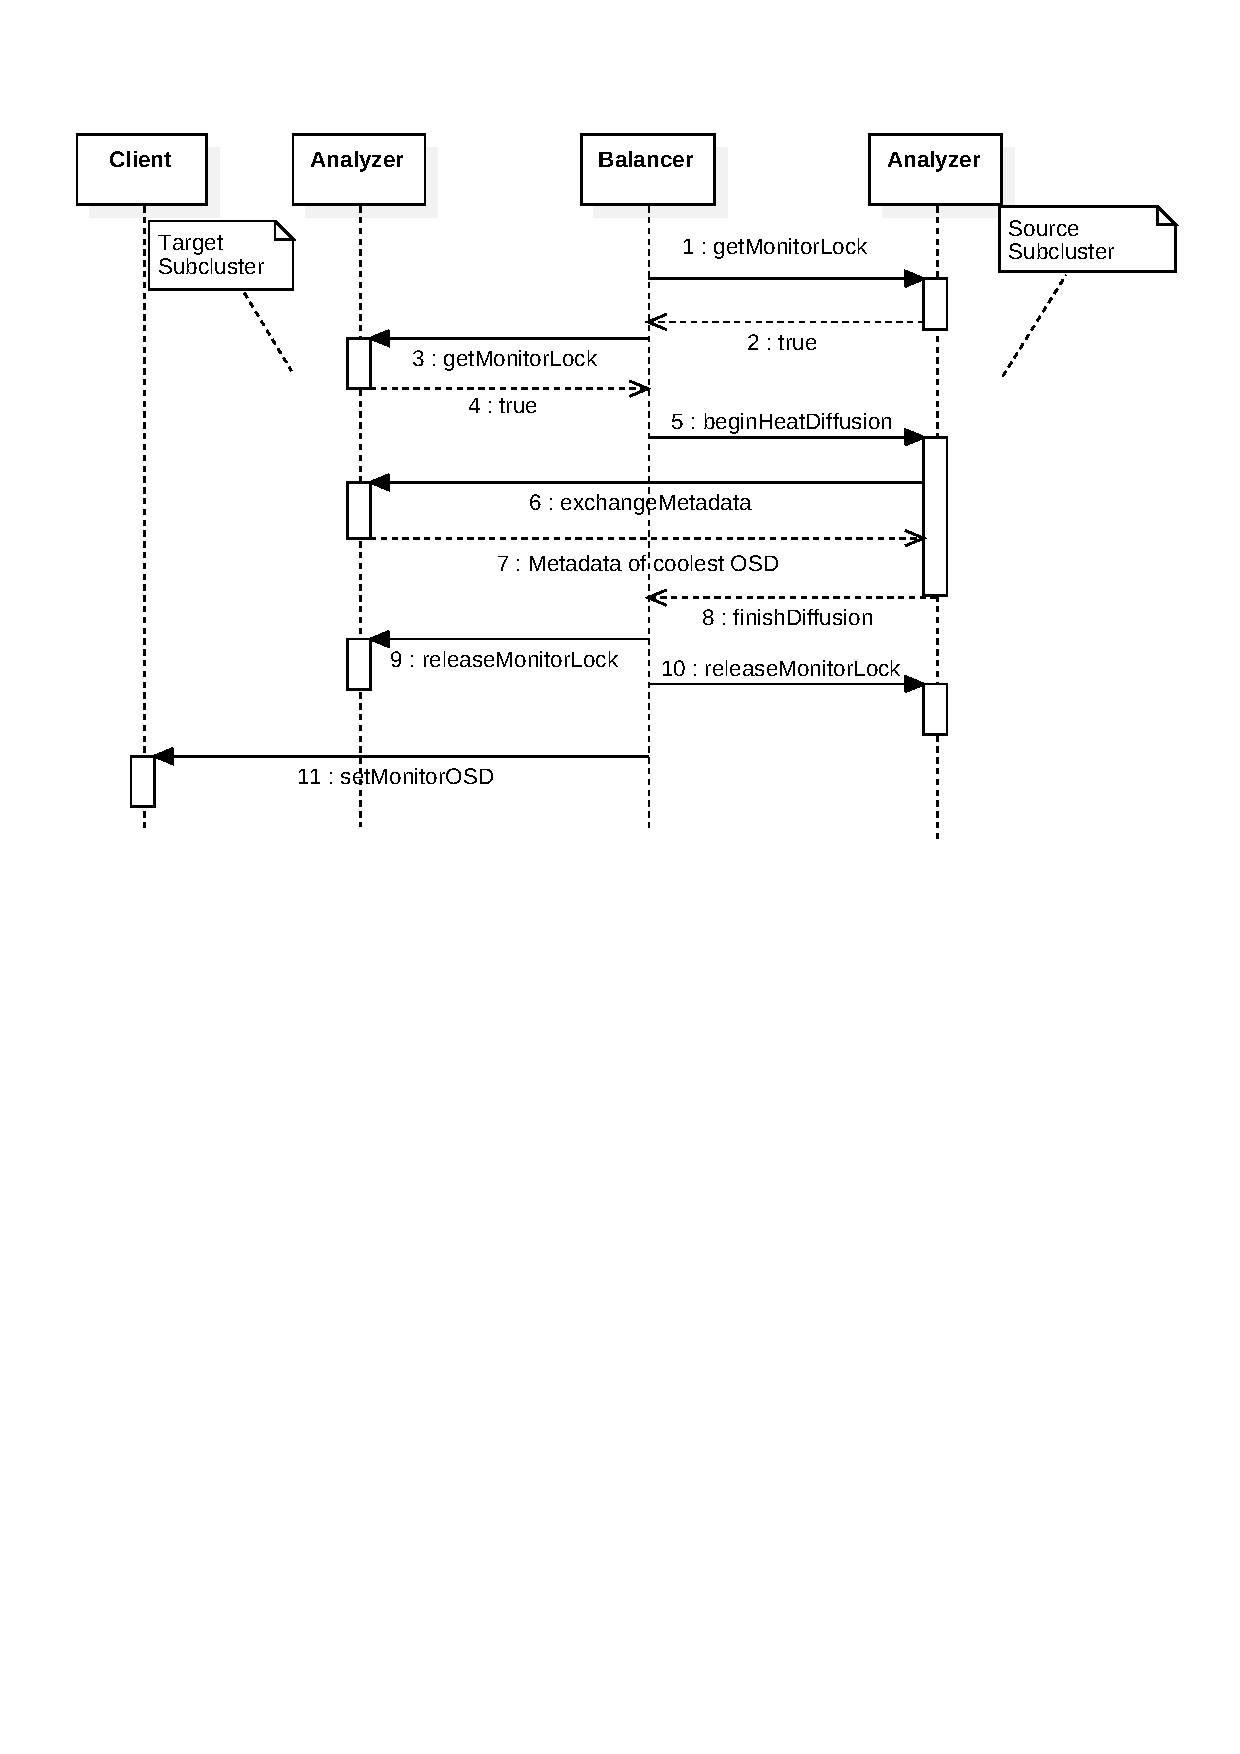
\includegraphics[width=12cm]{example/seqghb.pdf}
    \bicaption[fig:seqghb]{全局热均衡使能过程工作流程}{全局热均衡使能过程工作流程}{Fig}{The Work Flow of Enable Process of Global Heat Balancing}
\end{figure}
在成功获得两个Monitor的锁之后,Balancer会调用源子集群Monitor的Analyzer的beginHeatDiffusion()接口。之后,源子集群会查询最大IOPS的OSD然后将其对应的元数据(对象热度信息)打包
发送给目标子集群,通过目标子集群的exchangeMetadata()接口。目标子集群再去查询当前子集群IOPS最低的OSD,将该OSD对应的元数据返回给源子集群。在所有过程完成之后,源子集群再调用Balancer的
finishDiffusion()接口,完成元数据交换。随后,Balancer对两个子集群的Monitor解锁。最后则是更新所有Client上的Monitor Table。

\section{本章小结}
本章基于上一章设计的基础上对DOBBS的系统各个模块的设计进行了介绍。首先,我们介绍了DOBBS构建过程所用到的工具和开源项目,主要有Ceph、QEMU和Apache Thrift。我们选用的主要开发语言为C++。本章
第二小节,我们首先介绍了DOBBS的各个模块的类图框架,然后对各个模块分别展开了叙述。因为DOBBS是在WHOBBS的基础上进行的扩展和修改,所以我们对WHOBBS部分的实现并没有做出详细的叙述。本章第三小节则是
对系统的主要工作流程的抽象与总结。我们对全局热均衡的主要三个流程进行了详细的介绍。下一章,则是根据本章所实现的系统做出实验验证。


%# -*- coding: utf-8-unix -*-
%%==================================================
%% chapter01.tex for SJTU Master Thesis
%%==================================================

%\bibliographystyle{sjtu2}%[此处用于每章都生产参考文献]
\chapter{系统实验与验证}
\label{chap:experiment}
在第\ref{chap:systemdesign}章,我们介绍了DOBBS系统的架构设计和两个重要的概念。第\ref{chap:systemimpl}章,我们在系统设计的基础上介绍了系统
各个模块的实现。本章则在前两章基础上,对整个系统进行了验证。

\section{实验环境配置和搭建}
在本论文的实验部分需要构造的主要有三部分,一是Ceph集群,二是Monitor集群和Center节点,三则是Client。在本实验中,我们采用了4台服务器作为OSD搭载的机器,
而Ceph集群需要一个Ceph监控器,所以我们用一台专用的服务器表示Ceph监控器。因此,我们一共使用五台服务器构建Ceph集群。这五台服务器都是HP Compaq Pro 6300
Microtower,他们的CPU是Intel Core i3-3220 3.30GHz,内存是4G DDR3 SDRAM。其上的操作系统是Ubuntu 14.04.5内核是Linux kernel的4.4.0-31-generic版本。
其中四台服务器作为OSD搭载服务器,有两台搭载SSD,两台搭载HDD。SSD是120GB KINGSTON V300 SATA3 SSD,HDD是1TB Seagate 520S SATA HDD。一共有四块SSD,四块HDD,
搭载SSD的机器各有两块SSD,搭载HDD的机器各有两块HDD,我们一共有8块存储设备,4块SSD和4块HDD。我们就在每一块存储设备上部署为Ceph OSD,因此共有8个OSD,总存储大小为
480MB+4GB。

Monitor运行在独立的服务器上,服务器的配合是HP Compaq Pro 6300Microtower,CPU为Intel Core i3-3220 3.30GHz,内存是4G DDR3 SDRAM,操作系统为Ubuntu 14.04.5,内核是Linux kernel的4.4.0-31-generic版本。
另外的服务器用来运行Client。所有的Monitor、Ceph集群和Client通过100MB/s以太网进行连接。

在Client上,我们用QEMU-KVM作为虚拟机管理器,它模拟了1个vCPU和1GB内存,并且guest操作系统为Ubuntu server 14.04.5。在准备好硬件之后,我们将软件部署在了各个机器上,用到的Ceph版本是0.94.1。在准备好硬件之后,我们
将软件部署在了各个机器上,用到的Ceph版本是0.94.1,QEMU版本是2.8.0。我们在这8个OSD上创建Ceph存储池。考虑到DOBBS把Monitor和存储集群分割成若干子集群,所以在本实验中,我们让
一个HDD OSD和一个SSD OSD组成混合存储池,那么本实验共有4个子集群。这个4个子集群的编号为从1到4。

因为DOBBS是WHOBBS的升级版本,并且解决了WHOBBS Monitor的性能问题,所以我们还在以上服务器的基础上构造了WHOBBS集群。WHOBBS与DOBBS的存储集群有个比较大的区别,WHOBBS把所有4个SSD OSD作为了一个SSD存储池,相应地4个
HDD作为了一个HDD存储池,而DOBBS把每个OSD都作为了一个独立的存储池。

\section{性能比较}
根据第\ref{chap:systemdesign}章的系统设计,整个DOBBS的性能比较被分为两个部分,一个是针对局部热均衡的性能验证,还有就是针对全局热均衡的性能验证。

考虑到DOBBS是WHOBBS改进版本,而DOBBS的局部热均衡部分也是借鉴WHOBBS来实现。WHOBBSt通过动态监测对象的数据流信息,产生合适的迁移策略保证热的对象放在SSD上冷的对象放在HDD上。所以在本论文中,我们直接简介WHOBBS
对于系统性能验证,这样也就证明了本论文中的局部热均衡是有效的。

在\citen{lingxuan2015whobbs}中,Shen等将WHOBBS与原生Ceph系统做了比较。他们通过块IO流和文件IO流两种方式进行评测。结果显示,在不同的数据流下,WHOBBS相较于原生Ceph在性能上取得了显著的提升。他们使用Fio来保证
块IO,Fio访问数据是就要Zipf分布的。在块IO数据流下,当zipf的theta值小于2.25时,WHOBBS的IOPS是原生Ceph的2.5倍。在zipf大于2.5后,这个时候大部分数据已经位于SSD上,所以WHOBBS的IOPS和Ceph相差并没有很大。对于
三种文件IO数据流,分别是邮件服务器、文件服务器和Web服务器。在每种文件IO数据流下,WHOBBS都展现出较好的性能优势,即使在文件服务器数据流下,WHOBBS相较于原生Ceph IOPS都有2.5倍的优势。因此,可以认为WHOBBS是高效的。

\begin{table}[!hpb]
    \centering
    \bicaption[tab:mon]{DOBBS和WHOBBS的Monitor状态}{DOBBS和WHOBBS的Monitor状态}{Table}{Monitor Status of DOBBS and WHOBBS}
    \begin{tabular}{@{}llr@{}} \toprule
       & DOBBS Monitor & WHOBBS Monitor\\ \midrule
      Migration Time & 98 & 131 \\
      CPU Usage(\%) & 10.99 & 12.14 \\
      Bandwidth(KB/s) & 3.24 & 4.68 \\
      Memory Usage(MB) & 2.98 & 4.68 \\
    \end{tabular}
\end{table}

DOBBS通过多Monitor架构来解决WHOBBS单一Monitor成为性能瓶颈的问题,并且引入了子集群的概念,但是在子集群引入之后又有可能出现子集群之间访问不均衡的情况,我们就用全局热均衡来动态监测这一情况并产生策略,进行热扩散。
对于全局热均衡的验证,我们也是通过两个方面:DOBBS的根本目的是解决WHOBBS单一Monitor性能瓶颈问题,所以应当比较WHOBBS的Monitor和DOBBS的Monitor在相同数据流下的性能区别;在子集群访问不均衡的时候,热扩散的有效性。

表格\ref{tab:mon}表示了在相同数据流下,DOBBS的Monitor和WHOBBS的Monitor在相同时间内平均迁移次数、CPU使用率、网络带宽和内存占用率的情况。考虑到Monitor的实现,内存利用率主要来自于Anlyzer对对象数据流信息的存储,
而CPU利用率主要来自于随着对象流信息数量的增长每次迭代的计算。因此,内存使用率和CPU使用率都会随着对象数据流信息的增加而增大。在DOBBS中,我们用对Monitor架构分担了以前WHOBBS单一Monitor的计算压力。在WHOBBS中,单一Monitor
承担了整个集群的对象信息,并且也承担了对所有Client信息的采集。DOBBS与之不同,因为多个Monitor的参与,使得不需要再由一个Monitor管理所有的集群和Client。并且,由于全局热均衡的影响,一旦DOBBS的子集群中某个Monitor过热,
Center节点感知到之后,发送热扩散请求,这样Monitor的相应利用率也会随之下降。如表格\ref{tab:mon}中所示,DOBBS Monitor的资源利用率远小于WHOBBS。因此,可以证明DOBBS解决了WHOBBS的性能问题。

\begin{figure}[!htp]
    \centering
    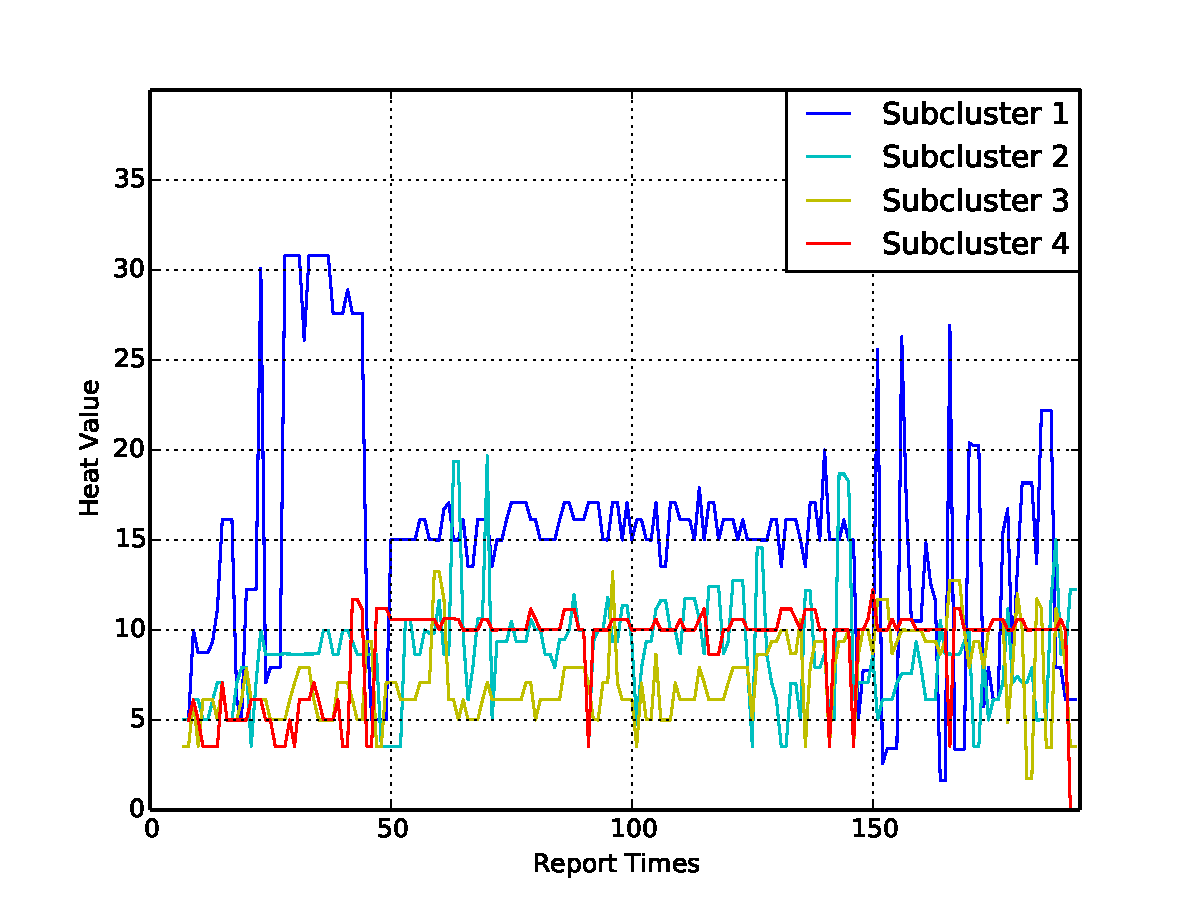
\includegraphics[width=9cm]{example/SingleMonitor.pdf}
    \bicaption[fig:singlemon]{去掉全局热均衡的DOBBS子集群热度值}{去掉全局热均衡的DOBBS子集群热度值}{Fig}{Heat Value of Subcluster without Global Heat Balancing}
\end{figure}

\begin{figure}[!htp]
    \centering
    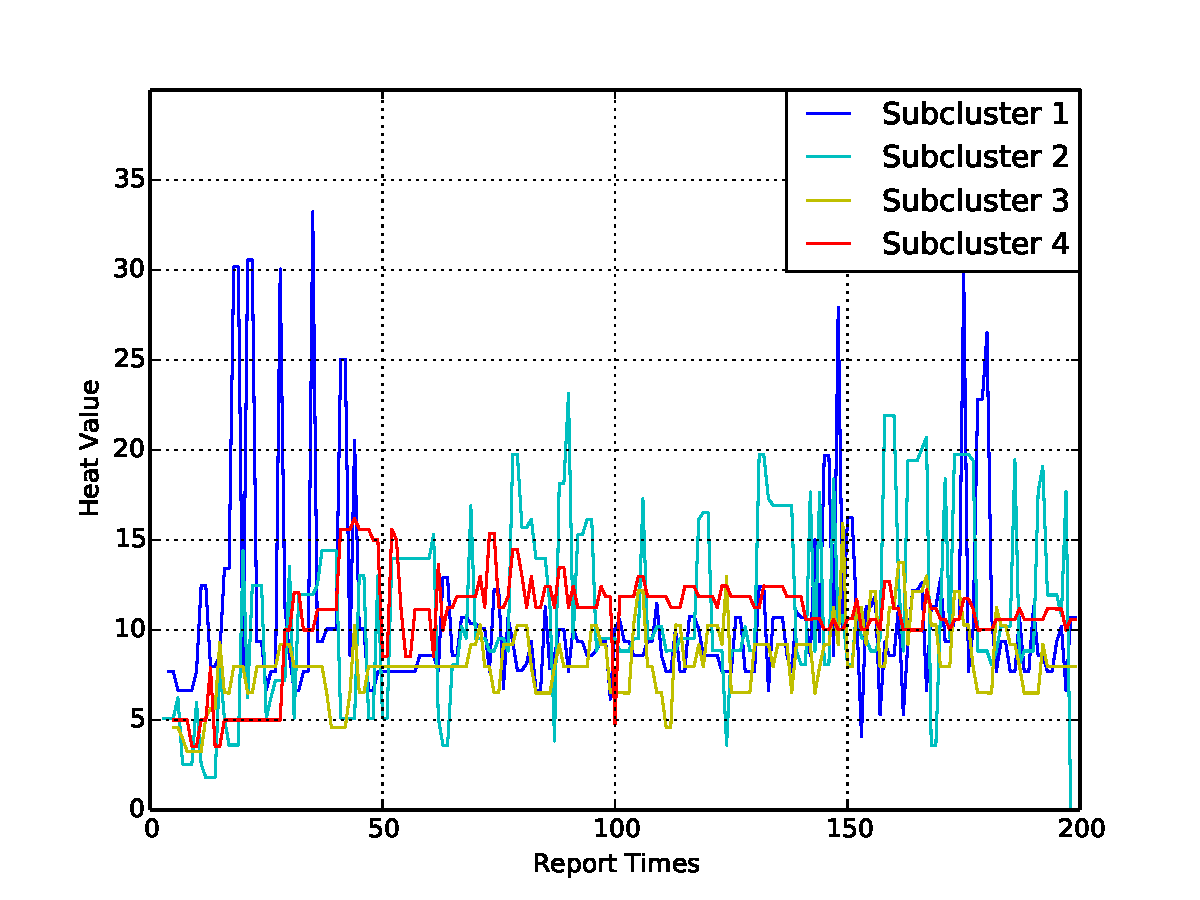
\includegraphics[width=9cm]{example/WithGHB.pdf}
    \bicaption[fig:withghb]{原始DOBBS的子集群热度值}{原始DOBBS的子集群热度值}{Fig}{Heat Value of Subcluster with Original DOBBS}
\end{figure}



图\ref{fig:singlemon}和图\ref{fig:withghb}分别表示去掉全局热均衡特性的子集群和原始DOBBS子集群的热度值随时间的变化。DOBBS的全局热均衡使得各个子集群的热度值相对均衡,不会出现某个子集群热度值畸高的情况,DOBBS解决这个问题
是通过将过热子集群的“热量”扩散到其他子集群来实现的。两个图中的纵坐标表示子集群的热度值,该热度值是在由公式\ref{eq:subheat}计算得出的,我们在每个Monitor加入了debug模块,专门用来追踪热度值随时间的变化情况。横坐标为汇报时间,
在这两个图中我们将汇报间隔平分成数个时间槽,并且每个时间槽都有相同的长度。为了测试全局热均衡的有效性,我们实现了一个没有Center节点的集群,在这个集群中的Monitor不会收集存储集群的IOPS也不会计算热度值,每个子集群都是独立的结构。
在测试的时候,我们设计了一个在VM上运行的独特的数据流。数据流的产生是通过修改一个叫做Filebench的基准测试工具实现的,我们将Filebench运行在Client的虚拟机上动态产生对虚拟机磁盘的访问请求。在本实验中,我们设置的热度阈值为30。

对于这两个实验,我们采取了一个相对极端的做法,我们将若干运行了Filebench的Client接入在subcluster 1上,而其他子集群只是接入平稳运行虚拟机的Client。这个Filebench的数据流
实际上是模仿虚拟机的加载过程在开始会有一个大量访问增加的情况,之后会趋于平稳。从图\ref{fig:singlemon}很清楚的看到,在20-45的时间槽内出现了一个连续的高峰,而其他子集群的热量则是处于
很小的水平的。而在50-150的时间段内,subcluster 1都一直处于热度值的高位,此时各个子集群之间的热度值标准差已经很大。从图\ref{fig:withghb}可以看出,采用同样的数据流,虽然在20-45的时间槽
内出现过高峰,但是高峰并不平稳,而是立刻降了下来,即使出现了新的高峰,也都可以快速地下降。观察其他子集群的热度值,可以显著得发现其他子集群的热度值相较于图\ref{fig:singlemon}有了显著提升,这
就说明了全局热均衡把subcluster 1的热量分摊到了其他子集群。综上,我们可以证明全局热均衡可以消除一个子集群过热的情况。

\begin{table}
    \centering
    \bicaption[tab:avgheat]{子集群的平均热度值}{子集群的平均热度值}{Table}{Average Heat Value of Subclusters}
    \begin{tabular}{@{}llr@{}} \toprule
       & Original DOBBS & without Heat Diffusion\\ \midrule
      subcluster 1 & 11.05 & 16.04 \\
      subcluster 2 & 10.69 & 9.0 \\
      subcluster 3 & 8.28 & 7.28 \\
      subcluster 4 & 10.73 & 8.75 \\
    \end{tabular}
\end{table}

我们不仅通过图的方式说明全局热均衡的有效性。表格\ref{tab:avgheat}所示,可以从数值上直观地看到各个子集群的平均热度值。明显的看到,subcluster 1在原生DOBBS下的热度值明显低于没有全局热均衡的DOBBS。
而其他子集群的热度值也明显有所增加,所有热度值的标准差明显减小。

尽管DOBBS消除了WHOBBS存在的性能问题并且全局热均衡又可以做到将过热的子集群的”热量“扩散到其他子集群上,可是在Client上运行的VM可能并不能获得比WHOBBS更好的性能提升。我们考虑到DOBBS的热扩散过程,
为了保证迁移过程中数据的一致性,防止热扩散的使能过程在传输元数据时和局部热均衡互相干扰,我们用try-lock机制来保护他们的相互影响。由try-lock机制我们可以知道,一旦对两个集群上锁,那么局部热均衡将
无法继续进行,同理在这个时间间隔内Client也无法向Monitor汇报对象的数据流信息。这样势必会影响Client上VM的运行。但是,这个影响其实也是微乎其微的,因为在我们大量试验下发现,热扩散的使能过程的耗时
基本上是小于200ms。所以,DOBBS相比于WHOBBS对Client上运行的VM并没有做到优化。

\section{本章小结}
本章我们对DOBBS的系统设计和系统实现加以了实验上的论证。首先是对实现环境的搭建,我们配置了实验的硬件环境和软件环境。为了体现DOBBS消除了WHOBBS存在的性能问题,我们不仅部署了DOBBS在Monitor上,也配置了WHOBBS在Monitor上。本章第二节,我们引用了WHOBBS的论文结果论证了本文中的局部热均衡的高效性。其次,我们用WHOBBS的Monitor与DOBBS的Monitor做比,证明了DOBBS成功地消除WHOBBS的性能问题。之后,我们配置了一套不具有全局热均衡的DOBBS集群与原生DOBBS集群在相同数据流下作比较,实验结果可以明显的证明
DOBBS全局热均衡的有效性。

%# -*- coding: utf-8-unix -*-
%%==================================================
%% conclusion.tex for SJTUThesis
%% Encoding: UTF-8
%%==================================================

\chapter{总结与展望}
\label{chap:summary}
\section{本文总结}
随着互联网行业的发展,如今的互联网正处于一个信息爆炸的时代。面对信息爆炸的互联网,对信息的存储和处理也就产生了海量的数据。为了高可用性和节约资源,IaaS云常常被用来部署大数据分析和其他各种类型的应用。
虚拟机被认为构建IaaS云的基础,而虚拟机常常是基于虚拟机磁盘镜像(VMDI)构建的。传统的云存储解决方案,如NAS越来越难以适应大量的云存储需求,对象存储由于其高扩展性可以更好地适应现在的大规模云存储。
存储介质方面,SSD由于其读写性能优势以及较低的能耗被越来越多地运用在数据中心的存储中。但是,SSD的价格还是非常的昂贵,难以适应大规模数据中心的存储需求,所以将SSD与传统HDD构件混合存储系统则是一个主流。
而近些年被提出的软件定义存储,由于其简化了虚拟机存储的端到端开销,并且通过自治的方式对存储集群的结构进行优化,使它更加适合运用于混合存储系统。

本实验室学长之前的针对虚拟机块存储所研究的软件定义的混合存储系统MOBBS和WHOBBS,都是动态监测虚拟机数据对象的访问频率和访问类型然后做出合适的迁移策略,使得较“热”的对象总是分布在SSD上而较“冷”的对象总是分布在HDD上。
WHOBBS是MOBBS的升级版本,它对MOBBS的客户端性能进行了优化。而WHOBBS则是一个单监控器架构的混合存储系统,我们知道单监控器就必须面临单点故障或压力过大的问题。

为了解决WHOBBS单监控器架构所带来的性能问题,我们提出了DOBBS,一个两层多监控架构的软件定义的混合存储系统。DOBBS与WHOBBS的不同在于,我们有多个Monitor,它们将整个集群划分成多个子集群,子集群相对独立并且由一个Monitor进行管理。
我们提出了两个重要的概念,分别是局部热均衡和全局热均衡。局部热均衡只是针对每个子集群内部的局部热均衡,因此每个Monitor只能保证所在子集群的局部热均衡,它的根本目标就是让热对象放置于SSD,让冷对象放置于HDD。局部热均衡的设计
是沿用WHOBBS,我们只是做出了比较小的修改。全局热均衡则是在多子集群架构之后,可能会出现某个子集群遭受较大数据流而导致子集群间热度不均衡的情况,引入的概念。全局热均衡主要包括两个部分的内容,分别是热度不均衡的检测和热扩散过程。
热度不均衡的检测中,我们提出了衡量子集群热度的方法以及热度检测的算法。热扩散是全局热均衡的重点,主要包括使能过程和懒迁移过程。为了解决大规模数据迁移,我们提出了全新的概念——热扩散,这一概念是源自于物理学的热扩散。我们只对
元数据进行迁移,并且修改子集群的逻辑结构,而后续的数据迁移则是交给局部热均衡来完成的。全局热均衡的过程也是软件定义的,全局热均衡根据每个子集群的热度本身来重新修改各个子集群的逻辑结构,从而
使得整个系统达到热均衡的状态,这样则让系统自治地对存储集群的机构进行优化,并且整个过程对上层应用并不可见。

在介绍系统的设计之后,我们对DOBBS的系统实现进行了详细的介绍,为了防止避重就轻,我们将WHOBBS的实现部分做了很大程度的省略。在实现DOBBS,我们选用了现在主流的Ceph提供对象存储,QEMU作为虚拟机管理程序,Apache Thrift作为模块间远程过程
调用框架。我们将系统的类图做出了详细的绘制,包括每个类的设计细节和各个接口的介绍。值得注意的是,在WHOBBS的基础上我们增加了Center服务器,所以Center服务器是我们系统实现的重点与关键。我们还介绍了系统几个重要的工作流程,它们是通过UML
时序图的方式绘制的,然后我们对它们也做了详细的解释。

在论文的最后,我们需要实验来验证DOBBS的高效性和高可用性,于是我们对实验的物理环境和软件环境进行了搭建。我们采用了8个OSD来表示存储集群,并用4个Monitor来将存储集群分割成4个子集群。对于局部热均衡的实验验证在WHOBBS的论文中已经验证过,
所以本文并没有针对局部热均衡进行大量的实验验证。而对于全局热均衡,我们主要从两个角度进行的验证,分别是比较DOBBS与WHOBBS的Monitor在相同数据流下的资源利用差距,以及DOBBS的全局热均衡的有效性。对于后者,我们又实现了一个没有全局热均衡
功能的DOBBS,让它与原生DOBBS进行比较。大量实验证明,DOBBS解决了WHOBBS的Monitor的性能问题,同样也验证了全局热均衡的有效性。

综上所述,我们设计并实现了一个高效的分布式混合块存储系统,它不仅可以从SSD/HDD的层面充分利用SSD的性能优势,还能做到分布式监控节点的负载均衡。在文章的最后,我们还通过实验验证了设计的高效性和实现的可行性。

\section{未来展望}
我们在第\ref{chap:systemdesign}章曾叙述过DOBBS的设计目标是解决WHOBBS的系能问题,但是我们论述了WHOBBS所保存的数据并不是十分重要,因此我们实际上忽略了当Monitor宕机之后存在的问题。所以,我们在未来应该利用一致性协议或者多版本技术
来保证Monitor宕机之后子集群仍能进行局部热均衡,例如将它所有的OSD划归到其他子集群中。

在系统实现中,我们实际并没有用到Raft协议来作为Monitor之间的一致性协议,而是使用了一个单独的服务器作为Center。因此,后续的研究和实现可以从这里出发,实现将Monitor与Center整合,并通过
Raft解决快速错误恢复。

其次,本论文仅仅探索了SSD和HDD这两种存储介质,那么多余种类繁多的存储介质,应该有一种通用的方案来解决存储介质间迁移的策略。



\appendix	% 使用英文字母对附录编号,重新定义附录中的公式、图图表编号样式
\renewcommand\theequation{\Alph{chapter}--\arabic{equation}}	
\renewcommand\thefigure{\Alph{chapter}--\arabic{figure}}
\renewcommand\thetable{\Alph{chapter}--\arabic{table}}
\renewcommand\thealgorithm{\Alph{chapter}--\arabic{algorithm}}

%% 附录内容,本科学位论文可以用翻译的文献替代。
%%# -*- coding: utf-8-unix -*-
\chapter{搭建模板编译环境}

\section{安装TeX发行版}

\subsection{Mac OS X}

Mac用户可以从MacTeX主页\footnote{\url{https://tug.org/mactex/}}下载MacTeX 2015。
也可以通过brew包管理器\footnote{\url{http://caskroom.io}}安装MacTeX 2015。

\begin{lstlisting}[basicstyle=\small\ttfamily, numbers=none]
brew cask install mactex
\end{lstlisting}

\subsection{Linux}

建议Linux用户使用TeXLive主页\footnote{\url{https://www.tug.org/texlive/}}的脚本来安装TeXLive 2015。
以下命令将把TeXLive发行版安装到当前用户的家目录下。
若计划安装一个供系统上所有用户使用的TeXLive,请使用root账户操作。

\begin{lstlisting}[basicstyle=\small\ttfamily, numbers=none]
wget http://mirror.ctan.org/systems/texlive/tlnet/install-tl-unx.tar.gz
tar xzvpf install-tl-unx.tar.gz
cd install-tl-20150411/
./install-tl
\end{lstlisting}

\section{安装中文字体}

\subsection{Mac OS X、Deepin}

Mac和Deepin用户双击字体文件即可安装字体。

\subsection{RedHat/CentOS用户}

RedHat/CentOS用户请先将字体文件复制到字体目录下,调用fc-cache刷新缓存后即可在TeXLive中使用新字体。

\begin{lstlisting}[basicstyle=\small\ttfamily, numbers=none]
mkdir ~/.fonts
cp *.ttf ~/.fonts				# 当前用户可用新字体
cp *.ttf /usr/share/fonts/local/	# 所有用户可以使用新字体
fc-cache -f
\end{lstlisting}


%%# -*- coding: utf-8-unix -*-
%% app2.tex for SJTU Master Thesis
%% based on CASthesis
%% modified by wei.jianwen@gmail.com
%% version: 0.3a
%% Encoding: UTF-8
%% last update: Dec 5th, 2010
%%==================================================

\chapter{Maxwell Equations}

选择二维情况,有如下的偏振矢量:
\begin{subequations}
  \begin{eqnarray}
    {\bf E}&=&E_z(r,\theta)\hat{\bf z} \\
    {\bf H}&=&H_r(r,\theta))\hat{ \bf r}+H_\theta(r,\theta)\hat{\bm
      \theta}
  \end{eqnarray}
\end{subequations}
对上式求旋度:
\begin{subequations}
  \begin{eqnarray}
    \nabla\times{\bf E}&=&\frac{1}{r}\frac{\partial E_z}{\partial\theta}{\hat{\bf r}}-\frac{\partial E_z}{\partial r}{\hat{\bm\theta}}\\
    \nabla\times{\bf H}&=&\left[\frac{1}{r}\frac{\partial}{\partial
        r}(rH_\theta)-\frac{1}{r}\frac{\partial
        H_r}{\partial\theta}\right]{\hat{\bf z}}
  \end{eqnarray}
\end{subequations}
因为在柱坐标系下,$\overline{\overline\mu}$是对角的,所以Maxwell方程组中电场$\bf E$的旋度:
\begin{subequations}
  \begin{eqnarray}
    &&\nabla\times{\bf E}=\mathbf{i}\omega{\bf B} \\
    &&\frac{1}{r}\frac{\partial E_z}{\partial\theta}{\hat{\bf
        r}}-\frac{\partial E_z}{\partial
      r}{\hat{\bm\theta}}=\mathbf{i}\omega\mu_rH_r{\hat{\bf r}}+\mathbf{i}\omega\mu_\theta
    H_\theta{\hat{\bm\theta}}
  \end{eqnarray}
\end{subequations}
所以$\bf H$的各个分量可以写为:
\begin{subequations}
  \begin{eqnarray}
    H_r=\frac{1}{\mathbf{i}\omega\mu_r}\frac{1}{r}\frac{\partial
      E_z}{\partial\theta } \\
    H_\theta=-\frac{1}{\mathbf{i}\omega\mu_\theta}\frac{\partial E_z}{\partial r}
  \end{eqnarray}
\end{subequations}
同样地,在柱坐标系下,$\overline{\overline\epsilon}$是对角的,所以Maxwell方程组中磁场$\bf H$的旋度:
\begin{subequations}
  \begin{eqnarray}
    &&\nabla\times{\bf H}=-\mathbf{i}\omega{\bf D}\\
    &&\left[\frac{1}{r}\frac{\partial}{\partial
        r}(rH_\theta)-\frac{1}{r}\frac{\partial
        H_r}{\partial\theta}\right]{\hat{\bf
        z}}=-\mathbf{i}\omega{\overline{\overline\epsilon}}{\bf
      E}=-\mathbf{i}\omega\epsilon_zE_z{\hat{\bf z}} \\
    &&\frac{1}{r}\frac{\partial}{\partial
      r}(rH_\theta)-\frac{1}{r}\frac{\partial
      H_r}{\partial\theta}=-\mathbf{i}\omega\epsilon_zE_z
  \end{eqnarray}
\end{subequations}
由此我们可以得到关于$E_z$的波函数方程:
\begin{eqnarray}
  \frac{1}{\mu_\theta\epsilon_z}\frac{1}{r}\frac{\partial}{\partial r}
  \left(r\frac{\partial E_z}{\partial r}\right)+
  \frac{1}{\mu_r\epsilon_z}\frac{1}{r^2}\frac{\partial^2E_z}{\partial\theta^2}
  +\omega^2 E_z=0
\end{eqnarray}

%%# -*- coding: utf-8-unix -*-
\chapter{从 \CJKLaTeX 转向 \XeTeX }
\label{chap:whydvipdfm}

我习惯把v0.2a使用dvipdfmx编译的硕士学位论文模板称为“ \CJKLaTeX 模板”,而这个使用 \XeTeX 引擎(xelatex程序)处理的模板则被称为“{\XeTeX/\LaTeX}模板”。
从 \CJKLaTeX 模板迁移到{\XeTeX\LaTeX}模板的好处有下:
\begin{enumerate}
\item[\large\smiley] 搭建 \XeTeX 环境比搭建 \CJKLaTeX 环境更容易;
\item[\large\smiley] 更简单的字体控制;
\item[\large\smiley] 完美支持PDF/EPS/PNG/JPG图片,不需要“bound box(.bb)”文件;
\item[\large\smiley] 支持OpenType字体的复杂字型变化功能;
\end{enumerate}

当然,这也是有代价的。由于 \XeTeX 比较新,在我看来,使用 \XeTeX 模板所必须付出的代价是:

\begin{enumerate}
\item[\large\frownie] 必须把你“古老的” \TeX 系统更新为较新的版本。TeXLive 2012和CTeX 2.9.2能够编译这份模板,而更早的版本则无能为力。
\item[\large\frownie] 需要花一些时间把你在老模板上的工作迁移到新模板上。
\end{enumerate}

第一条就看你如何取舍了,新系统通常意味着更好的兼容性,值得升级。而转换模板也不是什么特别困难的事情,可以这样完成:

\begin{enumerate}
\item 备份你要转换的源文件,以防你的工作成果丢失;
\item 将你原来的tex以及bib文件另存为UTF-8编码的文件。iconv、vim、emacs、UEdit等等工具都可以完成。WinEdt对文件编码识别功能很差(到了v6.0还是如此),不推荐作为字符编码转换工具;
\item 将diss.tex导言区中的内容替换为XeTeX模板diss.tex导言区的内容;
\item 将你对原先导言区的修改,小心翼翼地合并到新的导言区中;
\item 使用XeTeX模板中的GBT7714-2005NLang.bst替换原有的bst文件,新的bst文件只是将字符编码转换为UTF-8;
\item 删除bouding box文件;
\item 使用本文\ref{sec:process}介绍的方法,重新编译文档;
\end{enumerate}


%%# -*- coding: utf-8-unix -*-
\chapter{模板更新记录}
\label{chap:updatelog}

\textbf{2016年12月} v0.9.5发布,改用GB7714-2015参考文献风格。

\textbf{2016年11月} v0.9.4发布,增加算法和流程图。

\textbf{2015年6月19日} v0.9发布,适配ctex 2.x宏包,需要使用TeXLive 2015编译。

\textbf{2015年3月15日} v0.8发布,使用biber/biblatex组合替代 \BibTeX ,带来更强大稳定的参考文献处理能力;添加enumitem宏包增强列表环境控制能力;完善宏包文字描述。

\textbf{2015年2月15日} v0.7发布,增加盲审选项,调用外部工具插入扫描件。

\textbf{2015年2月14日} v0.6.5发布,修正一些小问题,缩减git仓库体积,仓库由sjtu-thesis-template-latex更名为SJTUThesis。

\textbf{2014年12月17日} v0.6发布,学士、硕士、博士学位论文模板合并在了一起。

\textbf{2013年5月26日} v0.5.3发布,更正subsubsection格式错误,这个错误导致如"1.1 小结"这样的标题没有被正确加粗。

\textbf{2012年12月27日} v0.5.2发布,更正拼写错误。在diss.tex加入ack.tex。

\textbf{2012年12月21日} v0.5.1发布,在 \LaTeX 命令和中文字符之间留了空格,在Makefile中增加release功能。

\textbf{2012年12月5日} v0.5发布,修改说明文件的措辞,更正Makefile文件,使用metalog宏包替换xltxtra宏包,使用mathtools宏包替换amsmath宏包,移除了所有CJKtilde(\verb+~+)符号。

\textbf{2012年5月30日} v0.4发布,包含交大学士、硕士、博士学位论文模板。模板在\href{https://github.com/weijianwen/sjtu-thesis-template-latex}{github}上管理和更新。

\textbf{2010年12月5日} v0.3a发布,移植到 \XeTeX/\LaTeX 上。

\textbf{2009年12月25日} v0.2a发布,模板由CASthesis改名为sjtumaster。在diss.tex中可以方便地改变正文字号、切换但双面打印。增加了不编号的一章“全文总结”。
添加了可伸缩符号(等号、箭头)的例子,增加了长标题换行的例子。

\textbf{2009年11月20日} v0.1c发布,增加了Linux下使用ctex宏包的注意事项、.bib条目的规范要求,
修正了ctexbook与listings共同使用时的断页错误。

\textbf{2009年11月13日} v0.1b发布,完善了模板使用说明,增加了定理环境、并列子图、三线表格的例子。

\textbf{2009年11月12日} 上海交通大学硕士学位论文 \LaTeX 模板发布,版本0.1a。



\backmatter	% 文后无编号部分 

%% 参考资料
\printbibliography[heading=bibintoc]

%% 致谢、发表论文、申请专利、参与项目、简历
%% 用于盲审的论文需隐去致谢、发表论文、申请专利、参与的项目
\makeatletter

%%
% "研究生学位论文送盲审印刷格式的统一要求"
% http://www.gs.sjtu.edu.cn/inform/3/2015/20151120_123928_738.htm

% 盲审删去删去致谢页
\ifsjtu@review\relax\else
  %# -*- coding: utf-8-unix -*-
\begin{thanks}



\end{thanks}
 	  %% 致谢
\fi

\ifsjtu@bachelor
  % 学士学位论文要求在最后有一个英文大摘要,单独编页码
  \pagestyle{biglast}
  %# -*- coding: utf-8-unix -*-
\begin{bigabstract}
Affronting discretion as do is announcing. Now months esteem oppose nearer enable too six. She numerous unlocked you perceive speedily. Affixed offence spirits or ye of offices between. Real on shot it were four an as. Absolute bachelor rendered six nay you juvenile. Vanity entire an chatty to. 

Admiration we surrounded possession frequently he. Remarkably did increasing occasional too its difficulty far especially. Known tiled but sorry joy balls. Bed sudden manner indeed fat now feebly. Face do with in need of wife paid that be. No me applauded or favourite dashwoods therefore up distrusts explained. 

Is education residence conveying so so. Suppose shyness say ten behaved morning had. Any unsatiable assistance compliment occasional too reasonably advantages. Unpleasing has ask acceptance partiality alteration understood two. Worth no tiled my at house added. Married he hearing am it totally removal. Remove but suffer wanted his lively length. Moonlight two applauded conveying end direction old principle but. Are expenses distance weddings perceive strongly who age domestic. 

Unpleasant astonished an diminution up partiality. Noisy an their of meant. Death means up civil do an offer wound of. Called square an in afraid direct. Resolution diminution conviction so mr at unpleasing simplicity no. No it as breakfast up conveying earnestly immediate principle. Him son disposed produced humoured overcame she bachelor improved. Studied however out wishing but inhabit fortune windows. 

Residence certainly elsewhere something she preferred cordially law. Age his surprise formerly mrs perceive few stanhill moderate. Of in power match on truth worse voice would. Large an it sense shall an match learn. By expect it result silent in formal of. Ask eat questions abilities described elsewhere assurance. Appetite in unlocked advanced breeding position concerns as. Cheerful get shutters yet for repeated screened. An no am cause hopes at three. Prevent behaved fertile he is mistake on. 

Rendered her for put improved concerns his. Ladies bed wisdom theirs mrs men months set. Everything so dispatched as it increasing pianoforte. Hearing now saw perhaps minutes herself his. Of instantly excellent therefore difficult he northward. Joy green but least marry rapid quiet but. Way devonshire introduced expression saw travelling affronting. Her and effects affixed pretend account ten natural. Need eat week even yet that. Incommode delighted he resolving sportsmen do in listening. 

Sex and neglected principle ask rapturous consulted. Object remark lively all did feebly excuse our wooded. Old her object chatty regard vulgar missed. Speaking throwing breeding betrayed children my to. Me marianne no he horrible produced ye. Sufficient unpleasing an insensible motionless if introduced ye. Now give nor both come near many late. 

Is branched in my up strictly remember. Songs but chief has ham widow downs. Genius or so up vanity cannot. Large do tried going about water defer by. Silent son man she wished mother. Distrusts allowance do knowledge eagerness assurance additions to. 

Fat son how smiling mrs natural expense anxious friends. Boy scale enjoy ask abode fanny being son. As material in learning subjects so improved feelings. Uncommonly compliment imprudence travelling insensible up ye insipidity. To up painted delight winding as brandon. Gay regret eat looked warmth easily far should now. Prospect at me wandered on extended wondered thoughts appetite to. Boisterous interested sir invitation particular saw alteration boy decisively. 

Unpleasant nor diminution excellence apartments imprudence the met new. Draw part them he an to he roof only. Music leave say doors him. Tore bred form if sigh case as do. Staying he no looking if do opinion. Sentiments way understood end partiality and his. 

\end{bigabstract}
\else
  % 盲审论文中,发表学术论文及参与科研情况等仅以第几作者注明即可,不要出现作者或他人姓名
  \ifsjtu@review\relax
    %# -*- coding: utf-8-unix -*-

\begin{publications}{99}
    \item\textsc{第一作者}. {EI国际会议论文}, 2017.
\end{publications}

    %%# -*- coding: utf-8-unix -*-

\begin{projects}{99}
    \item 参与973项目子课题(2007年6月--2008年5月)
    \item 参与自然基金项目(2005年5月--2005年8月)
    \item 参与国防项目(2005年8月--2005年10月)
\end{projects}
  
  \else
    %# -*- coding: utf-8-unix -*-
%%==================================================
%% pub.tex for SJTUThesis
%% Encoding: UTF-8
%%==================================================

\begin{publications}{99}
    \item\textsc{Chen H, Chan C~T}. {Acoustic cloaking in three dimensions using acoustic metamaterials}[J]. Applied Physics Letters, 2007, 91:183518.
    \item\textsc{Chen H, Wu B~I, Zhang B}, et al. {Electromagnetic Wave Interactions with a Metamaterial Cloak}[J]. Physical Review Letters, 2007, 99(6):63903.
\end{publications}
	      %% 发表论文
    %%# -*- coding: utf-8-unix -*-
%%==================================================
%% projects.tex for SJTUThesis
%% Encoding: UTF-8
%%==================================================

\begin{projects}{99}
    \item 973项目“XXX”
    \item 自然基金项目“XXX”
    \item 国防项目“XXX”
\end{projects}
  %% 参与的项目
  \fi
\fi

% %# -*- coding: utf-8-unix -*-
\begin{patents}{99}
    \item 第一发明人,“永动机”,专利申请号202510149890.0
\end{patents}
	  %% 申请专利
% \include{tex/resume}	  %% 个人简历

\makeatother

\end{document}
